\chapter{二次函数}

\section{二次函数}
\subsection{函数的奇偶性}

在研究二次函数之前,我们先来研究函数的一个性
质——函数的奇偶性。

我们先来描绘$y=x^2$的图象。

先作出下面的数值表:

\begin{center}
\begin{tabular}{c|ccccccccccc}
    \hline
    $x$   &$\cdots$&   $-2$   &   $-1.6$   &   $-1$   &   $-0.5$   &   $0$   &   $0.5$   &   $1$   &   $1.5$   &   $2$   &   $\cdots$      \\
    \hline
       $y$  &$\cdots$ &   $4$   &   $2.25$   &   $1$   &   $0.25$   &   $0$   &   $0.25$   &   $1$   &   $2.25$   &   $4$   &   $\cdots$\\
       \hline
\end{tabular}
\end{center}

用表里各组对应值作为点的坐标,作出各个点,然后用
平滑的曲线把它们连结起来,就得出$y=x^2$的图象(图5.1),
这个图象叫做抛物线。函数$y=x^2$的图象,以后简称为抛物线
$y=x^2$。

\begin{figure}[htp]
    \centering
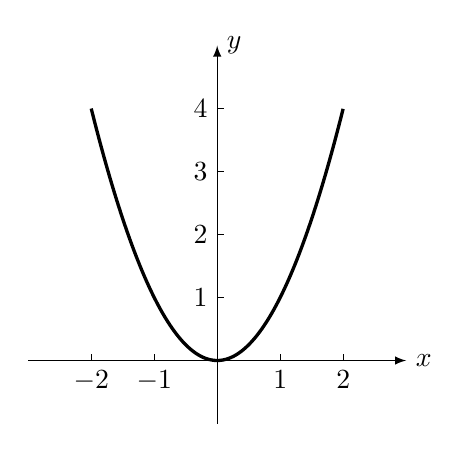
\begin{tikzpicture}[>=latex, scale=.8]
\draw[->](-3,0)--(3,0)node[right]{$x$};
\draw[->](0,-1)--(0,5)node[right]{$y$};
\foreach \x in {-2,-1,1,2}
{
    \draw (\x,0)node[below]{$\x$}--(\x, 0.1);
}
\foreach \x in {1,2,...,4}
{
    \draw (0,\x)node[left]{$\x$}--(.1,\x);
}

\draw[domain=-2:2, samples=100, very thick] plot(\x,{\x*\x});

\end{tikzpicture}
    \caption{}
\end{figure}


从上面表格中可以看到这个函数有一个特点:当自变量
取绝对值相等而符号相反的两个值时(如$x$取1.5和$-1.5$),
它们对应的函数值相等($y$都取2.25),这说明$y$轴垂直平分以
点$(x,f(x))$, $(-x,f(-x))$为端点的线段,换句话说,点
$(x,f(x))$, $(-x,f(x))$是关于$y$轴对称的,因此抛物线$y=x^2$
是关于$y$轴对称的。

我们把具有这种特征
的函数叫做偶函数。$f(x)$
是偶函数的标志是:当自
变量$x$取一对互为相反
数的值时,函数的值不
变,就有$f(x)=f(-x)$。

一般地说,对于函数
$f(x)$, 设$x$和$-x$都属于函
数的定义域,如果
\[f(-x)=f(x)\]
那么函数$f(x)$叫做\textbf{偶函数},偶函数的图象关于$y$轴对称。

我们再来画函数$y=\frac{1}{8}x^3$的图象

先作出下面的数值表:
\begin{center}
\begin{tabular}{c|ccccccccccc}
    \hline
    $x$ &$\cdots$&$-4$&$-3$&$-2$&$-1$&0&1&2&3&4&$\cdots$\\
\hline
$y$ &$\cdots$&$-8$&$-3\tfrac{3}{8}$&$-1$&$-\tfrac{1}{8}$&0&$\tfrac{1}{8}$&1&$3\tfrac{3}{8}$&8&$\cdots$\\
\hline
\end{tabular}
\end{center}

根据表里这些对应值,作出函数$y=x^3$的图象如图
5.2。这个图象称为立方抛物线。
\begin{figure}[htp]
    \centering
\begin{tikzpicture}[>=latex, scale=.5]
\draw[->](-5,0)--(5,0)node[right]{$x$};
\draw[->](0,-9)--(0,9)node[right]{$y$};
\foreach \x in {1,2,3,4}
{
    \draw (\x,0)node[below]{$\x$}--(\x, 0.1);
}
\foreach \x in {-2,-4}
{
    \draw (\x,0)node[above]{$\x$}--(\x, -0.1);
}
\foreach \x in {-8,-6,...,-2,2,4,...,8}
{
    \draw (0,\x)node[left]{$\x$}--(0.1,\x);
}
\node at (-.5,-.5){$O$};
\draw[domain=-4:4, samples=100, very thick] plot(\x,{\x*\x*\x/8});

\end{tikzpicture}
    \caption{}
\end{figure}

从上面表格中可以看到这个函数也有一个特征:因为,
$\frac{1}{8}(-x)^3=-\frac{1}{8}x^3$, 所以当自变量取两个互为相反数的值时,
对应的函数值也是互为相反数。所以如果点$(x,f(x))$在函
数的图象上,那么必有另一点$(-x,-f(x))$也在函数的图象
上,而原点恰是以$(x,f(x))$, $(-x,-f(x))$为端点的线段
的中点,换句话说,点$(x,f(x))$, $(-x,-f(x))$是关于原
点对称的。因此立方抛物线
$y=\frac{1}{8}x^3$是关于原点对称的,我
们把具有这种特征的函数叫做
奇函数,$f(x)$是奇函数的标志
是:当自变量$x$取一对互为相
反数的值时,函数的值也是
互为相反数,就是$f(-x)=-f(x)$。

一般地说,对于函数$f(x)$, 设$x$与$-x$都属于函数的定义
域,如果$$f(-x)=-f(x)$$ 那么函数$f(x)$叫做\textbf{奇函数}。奇函数的图象关于原点对称。

考虑一个函数是偶函数、奇函数,或者既不是偶函数又
不是奇函数,叫做研究函数的奇偶性,对于一个奇函数或者
偶函数,要了解它的性质和图象,只要了解当自变量取正
值时的性质和图象就可以了。例如,要作函数$y=\frac{1}{8}x^3$的图
象,因为它是奇函数,所以只要作出自变量取正值时的函数
图象,就可以利用奇函数的图象必定关于原点对称这一特点,
作出自变量取负值时的图象。

\begin{example}
研究下列函数的奇偶性:
\[f(x)=x^4+x^2,\qquad f(x)=x^3+x,\qquad f(x)=x+1\]   
\end{example}

\begin{solution}
\begin{enumerate}
    \item 对于$f(x)=x^4+x^2$, 我们有:
    \[f(-x)=(-x)^4+(-x)^2=x^4+x^2=f(x)\]
    $\therefore\quad $函数$f(x)=x^4+x^2$是偶函数。
    \item 对于$f(x)=x^3+x$, 我们有:
    \[f(-x)=(-x)^3+(-x)=-(x^3+x)=-f(x)\]
    $\therefore\quad $函数$f(x)=x^3+x$是奇函数。
    \item 对于$f(x)=x+1$, 我们有:
    \[f(-x)=-x+1\]
    这里$f(-x)\ne f(x)$, 并且$f(-x)\ne -f(x)$, 所以函数$f(x)=
x+1$既不是偶函数又不是奇函数。
\end{enumerate} 
\end{solution}

\begin{ex}
\begin{enumerate}
    \item  研究下面函数的奇偶性:(其中$k,b$是常数)
\begin{multicols}{2}
\begin{enumerate}
    \item $y=kx\quad (k\ne 0)$
    \item $y=\frac{k}{x}\quad (k\ne 0)$
    \item $y=kx+b\quad (k\ne 0)$
    \item $y=\sqrt{1+x^2}$
    \item $y=|x|$
    \item $y=\sqrt[3]{x}$
    \item $y=\sqrt{x}+1$
    \item $y=x^2+x+1$
\end{enumerate}
\end{multicols}
\item 证明:
\begin{enumerate}
    \item 两个偶函数的和是偶函数;
    \item 两个奇函数的和是奇函数;
    \item 两个偶函数的乘积是偶函数,
    \item 两个奇函数的乘积是偶函数;
    \item 偶函数与奇函数的乘积是奇函数。
\end{enumerate}
\end{enumerate}
\end{ex}

\subsection{函数$y=ax^2\; (a\ne 0)$的图象和性质}
在上一章里,我们研究了$x$的一次函数$y=ax+b$, 现在
我们要研究另一类重要的函数,这类函数的解析式是$x$的二
次式,我们把它叫做$x$的二次函数。

先看几个实例:

\begin{example}
    一石块离地面高为$h$, 设其速度为零,自由地落
到地面,运动的时间为$t$, 如果不考虑空气的阻力,于是$h$与
$t$之间将有函数关系:
\begin{equation}
 h=\frac{1}{2}gt^2   
\end{equation}
这里$g$是重力加速度。
\end{example}

\begin{example}
    农机厂第一个月水泵的产量为50(台),第三个月
的产量为$y$(台),与月平均增长
率之间的关系是:$y=50(1+x)^2$,即:
\begin{equation}
  y=50x^2+100x+50  
\end{equation}
\end{example}

\begin{example}
    设在半径是20厘米的
圆面上,从中心挖去一个半径为$x$厘米的圆面(图5.3),剩下的圆
环面积是$y$平方厘米,那么变量$y$和$x$间有下面的函数关系:
\begin{equation}
    y=400\pi-\pi x^2
\end{equation}
\end{example}

\begin{figure}[htp]
    \centering
\begin{tikzpicture}[>=latex]
 \draw [pattern=north east lines] (0,0) circle (1.5);
    \draw (0,0)[fill=white] circle (1);
\draw[->] (0,0)node[below]{$O$}--node[left]{$x$}(45:1);
\draw (0,0) -- (15:1.5);
\end{tikzpicture}    
    \caption{}
\end{figure}

从上面这些例子可以看出,它们有一个共同特点,那就
是每一个函数关系中,等号右边都是自变量的二次式。这些
函数都可以用
\begin{equation}
    y=ax^2+bx+c
\end{equation}
来表示,这里$a$是不等于零的实数,$b,c$是任意实数。

我们把函数$y=ax^2+bx+c\; (a\ne 0)$叫做$x$的二次函数。
下面我们先从最简单的情况开始研究,即研究在(5.4)中
取$b=0,c=0$的二次函数$y=ax^2\; (a\ne 0)$。

先来看$a>0$的情形。

我们已经在上一节和第三章中画过$y=x^2$和$y=\frac{1}{2}x^2$的图
象,现在把这两个图象和$y=2x^2$的图象都画在同一个坐标系
里。

先作下面的表:
\begin{center}
\begin{tabular}{c|ccccccccc}
    \hline
$x$ &$\cdots$ & $-2$  & $-\tfrac{3}{2}$  & $-1$   & 0   & 1&$\tfrac{3}{2}$& 2&$\cdots$\\
\hline
$y=2x^2$ &$\cdots$ & 8&$\tfrac{9}{2}$ &2  & 0   & 2&$\tfrac{9}{2}$ &8&$\cdots$\\
$y=x^2$ &$\cdots$ & 4&$\tfrac{9}{4}$&1  & 0   & 1&$\tfrac{9}{4}$&4&$\cdots$\\
$y=\tfrac{1}{2}x^2$ &$\cdots$ & $\tfrac{9}{8}$&$\tfrac{1}{2}$  & 0   & $\tfrac{1}{2}$  & $\tfrac{9}{8}$&2&$\cdots$\\
\hline
\end{tabular}    
\end{center}

\begin{figure}[htp]
    \centering
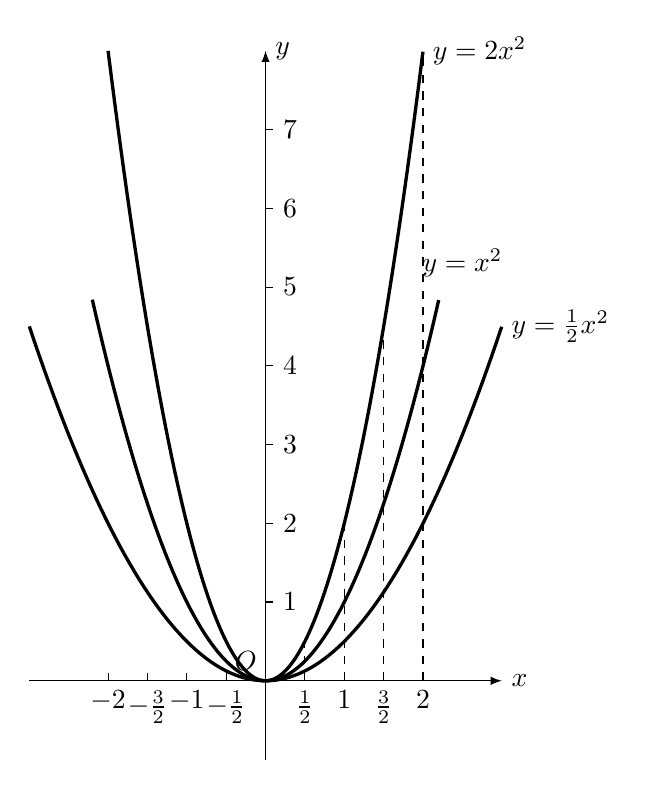
\begin{tikzpicture}[>=latex]
    \draw[->] (-3,0)--(3,0)node[right]{$x$};
    \draw [->] (0,-1)--(0,8)node[right]{$y$};
\foreach \y in {1,2,...,7}
{
    \draw (0,\y)--(.1,\y)node[right]{$\y$};
}
\foreach \x/\xtext in {-4/-2,-3/-\frac{3}{2},-2/-1,-1/-\frac{1}{2},1/\frac{1}{2},2/1,3/\frac{3}{2},4/2}
{
    \draw (\x/2,0)node[below]{$\xtext$}--(\x/2,.1);
}

\draw [domain=-3:3, samples=100, very thick]plot(\x,{\x*\x*0.5});
\draw [domain=-2.2:2.2, samples=100, very thick]plot(\x,{\x*\x});
\draw [domain=-2:2, samples=100, very thick]plot(\x,{\x*\x*2});
\node at (-.25,.25){$O$};
\foreach \x in {.5,1,...,2}
{
    \draw[dashed] (\x,0)--(\x,2*\x*\x);
}
\node at (2,8)[right]{$y=2x^2$};
\node at (2.5,5)[above]{$y=x^2$};
\node at (3,4.5)[right]{$y=\frac{1}{2}x^2$};
\end{tikzpicture}
    \caption{}
\end{figure}

从这个表可以看到,对于同一个$x$值,函数$y=2x^2$所对应
的值是函数$y=x^2$所对应的值的2倍。所以要画出函数$y=2x^2$
的图象,可以用$y=x^2$的图象为基础。

除了让这图象上的原点不动外,其它每一点的纵坐标都
拉长到原来的2倍,这样得到的新的点集就是$y=2x^2$的图象。
作图时我们只描出图象上几个关于$y$轴对称的点,如上表所
示,然后用平滑的曲线把它们连接起来。

同理,要作出函数$y=\frac{1}{2}x^2$的图象,也可以用$y=x^2$的图
象为基础。除了让$y=x^2$的图象上的原点不动外,其它每一点
的纵标都压缩到原来的$\frac{1}{2}$,便得到$y=\frac{1}{2}x^2$的图象。作图时
我们只描出图象上关于$y$轴对称的点,如上表所示,然后用
平滑曲线把它们连接起来。这样,就得到这三个函数的图象如图5.4。

再来看$a<0$的情形:

例如,我们要画函数$y=-x^2$的图象,也可以在函数$y=x^2$
的图象的基础上来研究。

作下面的表:
\begin{center}
\begin{tabular}{c|ccccccccc}
    \hline
$x$ &$\cdots$ & $-2$  & $-\tfrac{3}{2}$  & $-1$   & 0   & 1&$\tfrac{3}{2}$& 2&$\cdots$\\
\hline
$y=x^2$ &$\cdots$ & 4&$\tfrac{9}{4}$&1  & 0   & 1&$\tfrac{9}{4}$&4&$\cdots$\\
$y=-x^2$ &$\cdots$ & $-4$&$-\tfrac{9}{4}$&$-1$  & 0   & $-1$&$-\tfrac{9}{4}$&$-4$&$\cdots$\\
\hline
\end{tabular}    
\end{center}

从这个表可以看到,对于同一个$x$值,函数$y=-x^2$所对
应的值,恰巧是函数$y=x^2$所对应的值的相反数,当$x$遍取一
切实数值时,把函数$y=x^2$图象上的每一点纵坐标改为它的
相反数就得到函数$y=-x^2$的图象上的点,而以$(x,-x^2)$和
$(x,x^2)$为坐标的点是关于$x$轴的对称点,因此把图象$y=x^2$沿
$x$轴折转过来就可以得到$y=-x^2$的图象.$y=-x^2$的图象是在
$x$轴下方,开口向下(图5.5)。

同样,从函数$y=2x^2$和$y=4x^2$的图象可得出函数$y=
-2x^2$和$y=-4x^2$的图象(图5.6)。这些图象在x轴下方,开
口向下。

\begin{figure}[htp]\centering
    \begin{minipage}[t]{0.48\textwidth}
    \centering
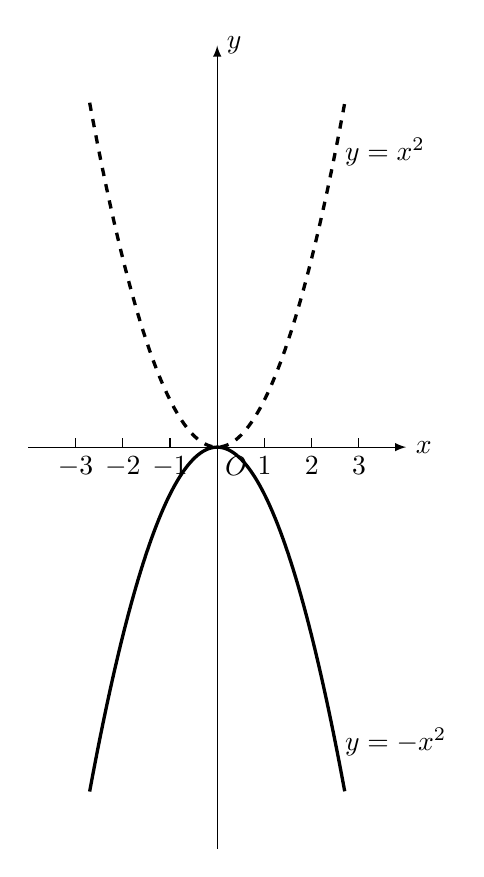
\begin{tikzpicture}[>=latex, scale=.6]
      \draw[->] (-4,0)--(4,0)node[right]{$x$};
    \draw [->] (0,-8.5)--(0,8.5)node[right]{$y$};

\foreach \x in {-3,-2,-1,1,2,3}
{
    \draw (\x,0)node[below]{$\x$}--(\x,.2);
}

\draw [domain=-2.7:2.7, samples=100, dashed, very thick]plot(\x,{\x*\x});
\draw [domain=-2.7:2.7, samples=100, very thick]plot(\x,{-\x*\x});
\node at (.4,-.4){$O$};
\node at (2.5,6.25)[right]{$y=x^2$};
\node at (2.5,-6.25)[right]{$y=-x^2$}; 
    \end{tikzpicture}
    \caption{}
    \end{minipage}
    \begin{minipage}[t]{0.48\textwidth}
    \centering
    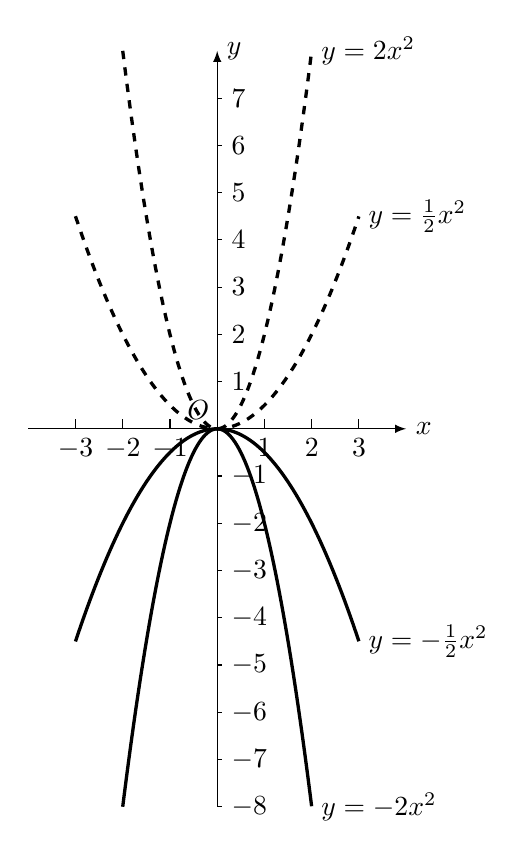
\begin{tikzpicture}[>=latex, scale=.6]
\draw[->] (-4,0)--(4,0)node[right]{$x$};
    \draw [->] (0,-8)--(0,8)node[right]{$y$};
\foreach \y in {-8,-7,...,-1,1,2,...,7}
{
    \draw (0,\y)--(.1,\y)node[right]{$\y$};
}
\foreach \x in {-3,-2,-1,1,2,3}
{
    \draw (\x,0)node[below]{$\x$}--(\x,.2);
}

\draw [domain=-3:3, samples=100, very thick, dashed]plot(\x,{\x*\x*0.5});
\draw [domain=-2:2, samples=100, very thick, dashed]plot(\x,{\x*\x*2});

\draw [domain=-3:3, samples=100, very thick]plot(\x,{-\x*\x*0.5});
\draw [domain=-2:2, samples=100, very thick]plot(\x,{-\x*\x*2});
\node at (-.4,.4){$O$};
\node at (2,8)[right]{$y=2x^2$};
\node at (3,4.5)[right]{$y=\frac{1}{2}x^2$};
\node at (2,-8)[right]{$y=-2x^2$};
\node at (3,-4.5)[right]{$y=-\frac{1}{2}x^2$};      
    \end{tikzpicture}
    \caption{}
    \end{minipage}
    \end{figure}

总结上面这两种情况,我们知道函数$y=ax^2$的图象是一
条抛物线。

从图象上我们能看到二次函数$y=ax^2$的下面一些性质:

\begin{blk}{性质1}
抛物线$y=ax^2$可向$x$轴左右方向无限延伸。这就是说
函数$y=ax^2$的定义域为实数集$\mathbb{R}$.
\end{blk}

\begin{blk}{性质2}
抛物线$y=ax^2$在$a>0$时,在$x$轴上方且在$y$轴的左
右两侧同时向上无限延伸,这就是说函数$y=ax^2$在$a>0$时,
函数值域为非负实数,即$\mathbb{R}^{+}\cup \{0\}$; 在$a<0$时,抛物线
$y=ax^2$在$x$轴下方且在y轴两侧同时向下无限延伸,这就是说
函数$y=ax^2$在$a<0$时,函数值域为非正实数,即$\mathbb{R}^{-}\cup \{0\}$.
\end{blk}

\begin{blk}{性质3}
抛物线$y=ax^2$在$a>0$时开口向上,在$a<0$时开口
向下,且$|a|$越大开口就越小。
\end{blk}

\begin{blk}{性质4}
抛物线$y=ax^2$关于$y$轴对称,这就是说函数$y=ax^2$是
个偶函数,事实上这个性质是可以证明的,即由于$f(-x)=
a(-x)^2=ax^2=f(x)$, 故函数$y=ax^2$是个偶函数.我们把$y$轴称
为抛物线$y=ax^2$的对称轴,其方程是$x=0$。
\end{blk}

\begin{blk}{性质5}
抛物线$y=ax^2$当$a>0$时,图象在$(-\infty,0)$是下
降的,在$(0,+\infty)$是上升的。这就是说函数$y=ax^2$当$a>0$
时,在$(-\infty,0)$是递减的;在$(0,+\infty)$是递增的(图5.7)。

抛物线$y=ax^2$当$a<0$时,图象在$(-\infty,0)$是上升的,
在$(0,+\infty)$是下降的,这就是说函数$y=ax^2$当$a<0$时,
在$(-\infty,0)$是递增的;在$(0,+\infty)$是递减的(图5.8)。
\end{blk}

\begin{figure}[htp]\centering
    \begin{minipage}[t]{0.48\textwidth}
    \centering
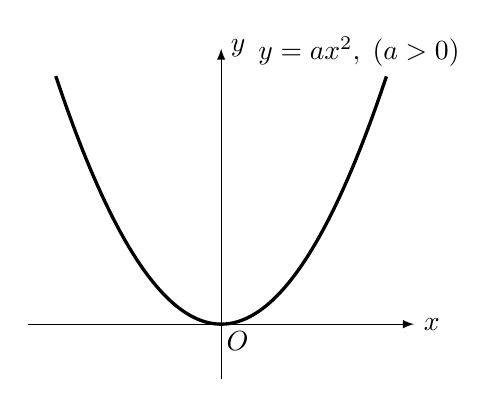
\begin{tikzpicture}[>=latex, scale=.7]
    \draw[->] (-3.5,0)--(3.5,0)node[right]{$x$};
    \draw [->] (0,-1)--(0,5)node[right]{$y$};
    \draw [domain=-3:3, samples=100, very thick]plot(\x,{\x*\x*0.5});
    \node at (2.5,4.5)[above]{$y=ax^2,\; (a>0)$};
    \node at (.3,-.3){$O$};
    \end{tikzpicture}
    \caption{}
    \end{minipage}
    \begin{minipage}[t]{0.48\textwidth}
    \centering
    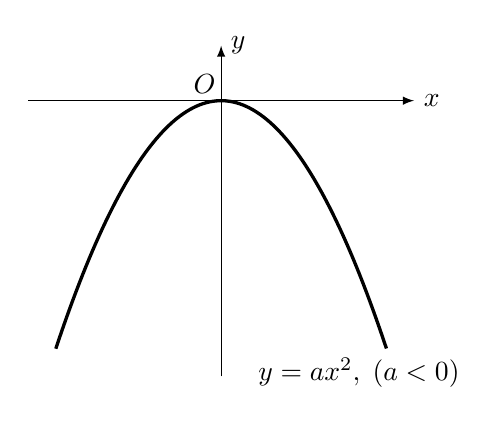
\begin{tikzpicture}[>=latex, scale=.7]
        \draw[->]  (-3.5,0)--(3.5,0)node[right]{$x$};
        \draw [->] (0,-5)--(0,1)node[right]{$y$};
        \draw [domain=-3:3, samples=100, very thick]plot(\x,{-\x*\x*0.5});    
    \node at (2.5,-4.5)[below]{$y=ax^2,\; (a<0)$};
    \node at (-.3,.3){$O$};
    \end{tikzpicture}
    \caption{}
    \end{minipage}
    \end{figure}

事实上,这个性质是可以证明的,我们只证$a>0$的情
况,$a<0$的情况留给同学们自己证明。

证明:函数 $y=ax^2$当$a>0$时,在$(-\infty,0)$是递减的,在$(0,+\infty)$是递增的。

\begin{proof}
\begin{enumerate}
    \item 设$x_1,x_2\in(-\infty,0)$且$x_1<x_2$,则
    \[\begin{split}
        f(x_2)-f(x_1)&=ax^2_2-ax^2_1=a(x^2_2-x^2_1)\\
&=a(x_2-x_1)(x_2+x_1)
    \end{split}\]
$\because \quad x_1,x_2\in(-\infty,0)$,$\therefore\quad x_1<0,\; x_2<0$

$\therefore\quad x_1+x_2<0$,又$a>0$,$x_2-x_1>0$

$\therefore\quad a(x_2-x_1)(x_2+x_1)<0$,则$f(x_2)<f(x_1)$

$\therefore\quad f(x)$在$(-\infty,0)$上递减。

    \item 设$x_1,x_2\in(0,+\infty)$且$x_1<x_2$,则
    \[f(x_2)-f(x_1)=a(x_2-x_1)(x_2+x_1)>0\]
    $\therefore\quad f(x_1)<f(x_2)$

$\therefore\quad f(x)$在$(0,+\infty)$上递增。
\end{enumerate} 

这样,在$a>0$的情况下,函数$y=ax^2$在$(-\infty,0)$上递减,而在$(0,+\infty)$上递增。
\end{proof}

\begin{blk}{性质6}
对称轴和抛物线的交点叫做抛物线的顶点。抛物线$y=ax^2$的顶点是原点$(0,0)$。这就是说,
有序数对$(0,0)$适合关系$y=ax^2$。
\end{blk}

\begin{blk}{性质7}
    抛物线$y=ax^2$的顶点的特点是:曲线由下降通过它转变到上升$(a>0)$,或者曲线由上升通过它转变到下降的一点$(a<0)$,相应地函数$f(x)=ax^2$($a>0$或$a<0$),在顶点横坐标$x_0=0$的左邻递减(递增),但是在$x_0=0$的右邻改为递增(递减),$x_0=0$是$f(x)=ax^2$在点$x_0=0$的邻近取极小
    (大)值的一点,我们称点$x_0=0$是$f(x)=ax^2$的一个极小(大)
    点,$f(0)=0$叫做$f(x)=ax^2$在极小(大)点$x_0=0$的极小(大)值。
\end{blk}



    在这里需要明确的是,极值都是函数由递增转到递减,或
    由递减转到递增的那一点取得的,而函数的最大值或最小
    值,仅仅指的是函数值的最大或最小,并不要求由递增到递
    减或由递减到递增的转变条件。

    由性质5知道,二次函数$y=ax^2$,仅有一个极值点$x_0=0$,
    在这种情形下,二次函数在点$x_0=0$的极值$f(0)=0$,与它
    的最大值或最小值是一致的。事实上,当$a>0$时,$y=ax^2$对
    于一切$x\in(-\infty,+\infty)$, 都有$f(x)=ax^2\ge 0$, 所以$f(0)=0$
    是最小值;当$a<0$时,$y=ax^2$对于一切$x\in(-\infty,+\infty)$, 都
    有$f(x)=ax^2\le 0$, 所以$f(0)=0$是最大值。对于二次函数,我
    们常用实数平方不小零这个原理来求一般二次函数的极值
    点和极值(也是二次函数的最值)。

从以上讨论可以看到,对抛物线$y=ax^2$主要要掌握三件
东西:对称轴、顶点、开口方向,即$a$的正负。而
这三件东西又都和二次函数的极值点、极值有关,顶点的坐
标确定后,对称轴方程和极值点也就随之求出,故顶点位置
是个关键。

最后我们要指出,上面我们是由抛物线$y=ax^2$的特点来
看二次函数$y=ax^2$的性质的,但今后等我们逐步地学到了更
多的函数性质后,我们应该有意识地学会先研究函数的性
质,再由函数的性质去把握函数图象的大致形状,最后用描
点法画出图象,这时所画的函数图象就较为精确了。


\begin{ex}
\begin{enumerate}
    \item 设从固定的半径$R$的圆板上,挖掉半径为$r$的同心圆板,
    问所剩圆环面积$S$与$r$之间的关系是什么?
    \item 用16m长的篱笆,围成一个一边靠墙的矩形养鸡场,如
    果与墙垂直的一边长是$x$m,面积是$y{\rm m}^2$, 则$x$与$y$之间
    有什么关系?
    \item     用一块矩形空地来做花圃,这块地长20m,宽15m,
    如在四周留出宽度都是$x$米的小路,中间余下种花的空
地面积是$y{\rm m}^2$, 则$y$与$x$之间有什么关系?
\item  汽车在前8秒钟内以匀加速度$a=0.8{\rm m/s}^2$行驶。
\begin{enumerate}
\item 利用公式$s=\frac{1}{2}at^2$, 求$t=3$(s),$t=5.5$(s), $t=2.5$(s) 时所行的路程$s$(m);
\item 画出$s$和$t$之间函数关系的图象;
\item 根据图象,求汽车走5m、10m、15m所需时间。
\end{enumerate}

\item  
在坐标纸上画出函数$y=x^2$图象:
\begin{enumerate}
\item 根据图象,求当$x=1.5$; $x=2.3$; $x=-1.4$时,$y$
的值(精确到0.1);
\item 根据图象,求当$y=2$; $y=3$; $y=4.5$时,对应
的$x$的值(精确到0.1);
\item 利用图象求$\sqrt{5}$, $\sqrt{7}$的值(精确到0.1)。
\end{enumerate}

\item   在同一坐标系里作以下函数的图象:
$$y=3x^2,\qquad y=3x^2,\qquad y=-3x^2,\qquad y=-\frac{1}{3}x^2$$
这些图象有哪些相同的地方?哪些不同的地方?
\item  试证当$a<0$时,二次函数$y=ax^2$在$(-\infty,0)$上递增,
而在$(0,+\infty)$上递减。
\item   证明抛物线$y=ax^2$与抛物线$y=x^2$是位似形。
\end{enumerate}
\end{ex}

\subsection{函数$y=ax^2+bx+c\; (a\ne 0)$的图象}
\subsubsection{函数$y=ax^2+c\; (a\ne 0)$的图象}
为确定起见,假设$c>0$, 从解析式$y=ax^2+c$和$y=ax^2$
明显地看出,对于自变量的相同值,$y=ax^2+c$的对应值,
总可以由$y=ax^2$的对应值加上$c$得到,这表示$y=ax^2+c$的图
象上的一切点比抛物线$y=ax^2$上具有相同横坐标的点高出$c$
个单位。因此,$y=ax^2+c$的图象,可以由抛物线$y=ax^2$沿着$y$
轴向上平移$c$个单位得到。如果$c<0$, 那么$y=ax^2+c$的图象是
由抛物线$y=ax^2$, 沿着$y$轴向下平移$|c|$个单位得到。

例如,我们把函数$y=2x^2$的图象向上移动1个单位,就
可以得到函数$y=2x^2+1$的图象;向下移动3个单位,就可
以得到函数$y=2x^2-3$的图象。

所以函数$y=ax^2+c$的图象仍旧是一条抛物线。当$a>0$时,
开口向上;$a<0$时,开口向下,对称轴方程是$x=0$($y$轴为
对称轴);顶点坐标是$(0,c)$。 当$a>0$时,在$x=0$处取得
$y_{\min}=c$。当$a<0$时,在$x=0$处取得$y_{\max}=c$(注:以后我们用
$y_{\min}$表示$y$的极小值;用$y_{\max}$表示$y$的极大值)。

我们从图形的平移观点确定了$y=kx+b$的图象是一条平
行于直线$y=kx$的直线,也确定了$y=ax^2+c$的图象是抛物线,
它的顶点是$(0,c)$。更一般的结论是:

函数$y=f(x)+b$的图象是由$y=f(x)$的图象沿$y$轴平移而
来的,若$b>0$, 则向上平移$b$个单位。若$b<0$, 则向下平移
$|b|$个单位。

\subsubsection{函数$y=a(x+m)^2$的图象}
例如函数$y=\frac{1}{4}(x+2)^2$, $y=\frac{1}{4}(x-2)^2$都是这种类型
的函数。

我们把上面两个函数的图象与$y=\frac{1}{4}x^2$比较。分别列表如下:
\begin{center}
\begin{tabular}{c|ccccccccccc}
\hline
    $x$ & $-5$& $-4$& $-3$& $-2$& $-1$& 0& 1& 2& 3& 4& 5\\
\hline
$y=\tfrac{1}{4}x^2$ &  $6\tfrac{1}{4}$   &  $4$  &  $2\tfrac{1}{4}$  &  $1$  &  $\tfrac{1}{4}$  &  $0$  &  $\tfrac{1}{4}$  &  $1$ & $2\tfrac{1}{4}$ &4&$6\tfrac{1}{4}$\\
$y=\tfrac{1}{4}(x+2)^2$& $2\tfrac{1}{4}$ &  $1$  &  $\tfrac{1}{4}$  & 0& $\tfrac{1}{4}$  & 1& $2\tfrac{1}{4}$ &4 &  $6\tfrac{1}{4}$  & 9& $12\tfrac{1}{4}$\\ 
$y=\tfrac{1}{4}(x-2)^2$& $12\tfrac{1}{4}$ &  $9$  &  $6\tfrac{1}{4}$  &  $4$  &  $2\tfrac{1}{4}$  &  $1$  &  $\tfrac{1}{4}$  &  $0$  &  $\tfrac{1}{4}$   &1 &  $2\tfrac{1}{4}$\\ 
\hline
\end{tabular}
\end{center}


\begin{figure}[htp]
    \centering
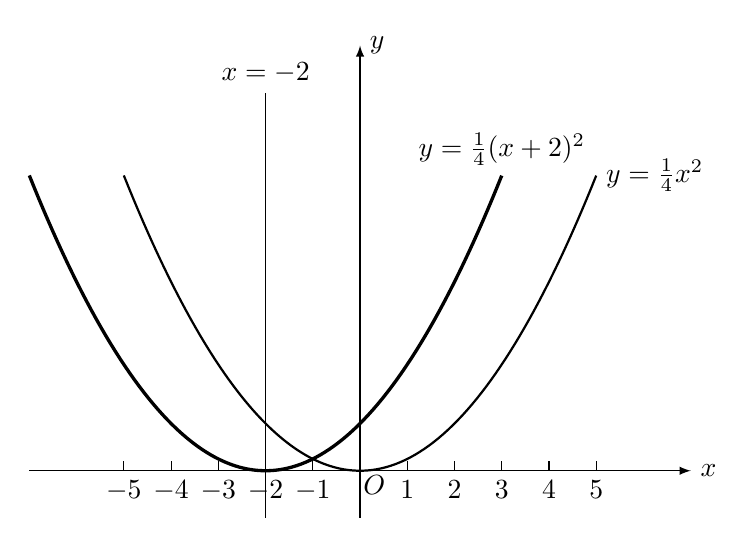
\begin{tikzpicture}[>=latex, scale=.6]
\draw[->] (-7,0)--(7,0)node[right]{$x$};
\draw[->] (0,-1)--(0,9)node[right]{$y$};
\foreach \x in {-5,-4,...,-1,1,2,...,5}
{
    \draw (\x,0)node[below]{$\x$}--(\x,.2);
}
\node at (.3,-.3){$O$};

\draw [domain=-5:5, samples=100, thick] plot(\x,{0.25*\x*\x});
\draw [domain=-7:3, samples=100, very thick] plot(\x,{0.25*(\x+2)*(\x+2)});
\draw (-2,-1)--(-2,8)node[above]{$x=-2$};
\node at (5,6.25)[right]{$y=\frac{1}{4}x^2$};
\node at (3,6.25)[above]{$y=\frac{1}{4}(x+2)^2$};
\end{tikzpicture}
    \caption{}
\end{figure}

从表中可以看出,函数$y=\frac{1}{4}(x+2)^2$在自变量取某一值
$x=x_1$时,所对应的函数值$y=\frac{1}{4}(x+2)^2$, 恰巧和函数$y=\frac{1}{4}x^2$在自变量取值$x=x_1+2$时所对应的函数值$y=\frac{1}{4}(x+2)^2$
相同.这就告诉我们,在函数$y=\frac{1}{4}(x+2)^2$的图象上的点
$\left(x_1,\frac{1}{4}(x_1+2)^2\right)$与函数$y=\frac{1}{4}x^2$的图象上的点$\left(x_1+2,\frac{1}{4}(x_1+2)^2\right)$的纵坐标相等,因此这两点的连接线段平行$x$轴,
并且横坐标是$x_1$的点在横坐标是$x_1+2$的点的右边2个单位
处,利用这个关系,我们只需把函数$y=\frac{1}{4}x^2$的图象上的每一
点向左平移2个单位,就可以得到函数$y=\frac{1}{4}(x+2)^2$的图象
(图5.9)。


同样,函数$y=\frac{1}{4}(x-2)^2$在自变量取某一值$x$时,所对
应的函数值$y=\frac{1}{4}(x_1-2)^2$, 恰巧和函数$y=\frac{1}{4}x^2$在自变量取
值$x=x_1-2$时,所对应的函数值$y=\frac{1}{4}(x_1-2)^2$相同,这就
告诉我们,在函数$y=\frac{1}{4}(x-2)^2$的图象上,横坐标是$x_1$的
点的纵坐标就等于函数$y=\frac{1}{4}x^2$的图象上横坐标是$x_1-2$的
点的纵坐标。利用这个关系,我们只需把函数$y=\frac{1}{4}x^2$的图象
上的每一点向右平移2个单位,就可以得到函数$y=\frac{1}{4}(x-2)^2$的图象(图
5.10)。

\begin{figure}[htp]
    \centering
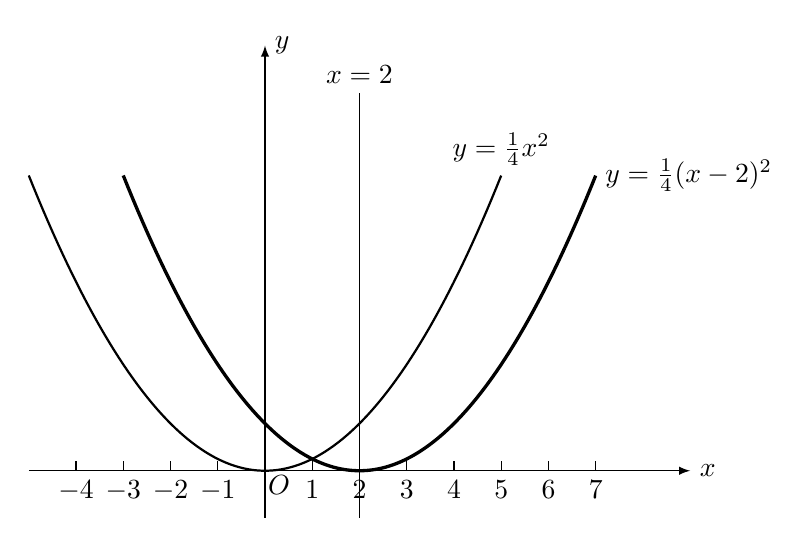
\begin{tikzpicture}[>=latex, scale=.6]
\draw[->] (-5,0)--(9,0)node[right]{$x$};
\draw[->] (0,-1)--(0,9)node[right]{$y$};
\foreach \x in {-4,-3,...,-1,1,2,...,7}
{
    \draw (\x,0)node[below]{$\x$}--(\x,.2);
}
\node at (.3,-.3){$O$};
\draw [domain=-5:5, samples=100, thick] plot(\x,{0.25*\x*\x});
\draw [domain=-3:7, samples=100, very thick] plot(\x,{0.25*(\x-2)*(\x-2)});
\draw (2,-1)--(2,8)node[above]{$x=2$};
\node at (5,6.25)[above]{$y=\frac{1}{4}x^2$};
\node at (7,6.25)[right]{$y=\frac{1}{4}(x-2)^2$};
\end{tikzpicture}
    \caption{}
\end{figure}


由此可见,函数$y=a(x+m)^2$的
图象,由函数$y=ax^2$的图象沿$x$轴方向左右平移得到。
当$m>0$时,向左平移$m$个单位;当$m<0$时,向右平
移$|m|$个单位。

因此函数$y=a(x+m)^2$的图象,仍然是一条抛物线,$a>0$
时,开口向上;$a<0$时,开口向下,对称轴方程是$x=-m$,
顶点坐标是$(-m,0)$. 当$a>0$时,在$x=-m$处取得$y_{\min}=0$, 当$a<0$时,在$x=-m$处取得$y_{\max}=0$。

应当指出:
\begin{enumerate}
    \item 上述的平移原理可以推广到一般情形。即函数$f(x+m)$的图象,是由函数$f(x)$的图象沿$x$轴方向左右平移得到。当
    $m>0$时,向左平移$m$个单位;当$m<0$时,向右平移$|m|$个单位。
    \item 具体作函数$y=a(x+m)^2$的图象时,不必先作出
    $y=ax^2\; (a\ne 0)$的图象,再作相应的平移得到它,而是先确
    定抛物线$y=a(x+m)^2$的顶点和对称轴,从顶点开始,左右
    取对称的点,再用平滑曲线去连接。
\end{enumerate}

\begin{example}
    作函数$y=2\left(x+2\frac{1}{2}\right)^2$的图象。
\end{example}

\begin{solution}
\begin{enumerate}
    \item 顶点坐标$\left(-2\frac{1}{2},0\right)$, 对称方程$x=-2\frac{1}{2}$,
    $a=2>0$, 开口向上。
    \item 列表:
\begin{center}
\begin{tabular}{c|ccccccccccc}
\hline
$x$&$\cdots$& $-4\tfrac{1}{2}$ &  $-4$ &  $-3\tfrac{1}{2}$ &  $-3$ &  $-2\tfrac{1}{2}$ &  $-2$ &  $-1\tfrac{1}{2}$ &  $-1$ &  $-\tfrac{1}{2}$ &$\cdots$\\
\hline
$y$&$\cdots$ & $8$& $4\tfrac{1}{2}$ &  $2$ &  $\tfrac{1}{2}$ &  $0$ &  $\tfrac{1}{2}$ &  $2$ &  $4\tfrac{1}{2}$ &  $8$ &  $\cdots$ \\
\hline
\end{tabular}
\end{center}

\item 完成图象如图5.11.
\end{enumerate}      

\begin{figure}[htp]
    \centering
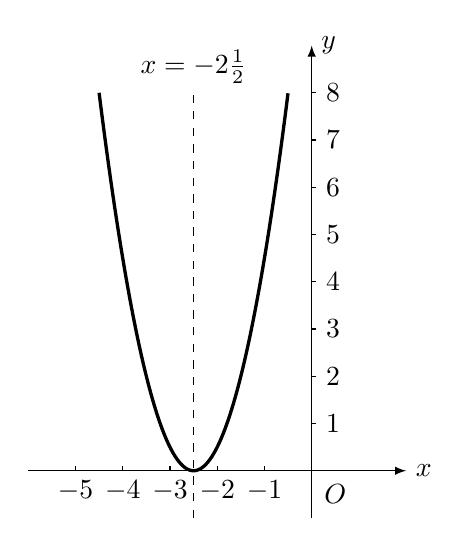
\begin{tikzpicture}[>=latex, scale=.6]
\draw[->] (-6,0)--(2,0)node[right]{$x$};
\draw[->] (0,-1)--(0,9)node[right]{$y$};
\foreach \x in {-5,-4,...,-1}
{
    \draw (\x,0)node[below]{$\x$}--(\x,.1);
}
\foreach \y in {1,2,...,8}
{
    \draw (0,\y)--(.1,\y)node[right]{$\y$};
}
\node at (.5,-.5){$O$};
\draw [domain=-4.5:-.5, samples=100, very thick]plot(\x, {2*(\x+2.5)*(\x+2.5)});
\draw[dashed](-2.5,-1)--(-2.5,8)node[above]{$x=-2\frac{1}{2}$};
\end{tikzpicture}
    \caption{}
\end{figure}
\end{solution}


\subsubsection{函数$y=-\frac{1}{4}(x-2)^2-3$的图象}

函数$y=a(x+m)^2+k$的图象,是由函数$y=a(x+m)^2$的图象
沿$y$轴方向上下平移得
到.当$k>0$时,向上平移$k$个
单位;当$k<0$时,向下平移
$|k|$个单位。而$y=a(x+m)^2$的
图象,是由$y=ax^2$的图象沿$x$轴
方向左右平移得到.当$m>0$
时,向左平移$m$个单位;当$m<0$时,向右平移$|m|$个单位,
故函数$y=a(x+m)^2+k$的图象,是由函数$y=ax^2$的图象经上
下左右平移得到。

由此可见,函数$y=a(x+m)^2+k$的图象,也是一条抛
物线,当$a>0$时,开口向上,当$a<0$时,开口向下.对称轴
方程是$x=-m$, 顶点坐标是$(-m,k)$. 当$a>0$时,在$x=
-m$处取得$y_{\min}=k$,当$a<0$时,在$x=-m$处取得$y_{\max}=k$。

\begin{example}
    研究函数$y=\frac{1}{4}(x+2)^2+3$的图象。
\end{example}

\begin{solution}
函数$y=\frac{1}{4}(x+2)^2+3$的图象,就是抛物线
$y=\frac{1}{4}(x+2)^2$向上平移3个单位,也就是抛物线$y=\frac{1}{4}x^2$向
左平移2个单位后,再向上平移3个单位。这条抛物线对你
轴方程是$x=-2$,开口向上,顶点坐标是$(-2,3)$. 在$x=-2$时,取得$y=3$。

\textbf{另解:}$\because\quad (x+2)^2\ge 0$

$\therefore\quad y=\frac{1}{4}(x+2)^2+3\ge 3$, 等式在$x=-2$时
成立,即在$x=-2$时,$y_{\min}=3$

由此得知抛物线$y=\frac{1}{4}(x+2)^2+3$的顶点是$(-2,3)$. 
对称轴方程是$x=-2$,它可以由抛物线$y=\frac{1}{4}x^2$向左平移2
个单位,再向上平移3个单位得来。
\end{solution}


\begin{example}
    作函数$y=-\frac{1}{4}(x-2)^2-3$的图象。
\end{example}

\begin{solution}
\begin{enumerate}
    \item 函数$y=-\frac{1}{4}(x-2)^2-3$的图象是抛物线。由
    $a=-\frac{1}{4}<0$知抛物线开口向下,顶点坐标是$(2,-3)$对称轴
    方程是$x=2$。
  \item 列表:
\begin{center}
\begin{tabular}{c|ccccccccccc}
\hline
$x$&$\cdots$& $-2$ &  $-1$ & 0 &  1 & 2 &  3 &  4 &  5 &  6 &$\cdots$\\
\hline
$y$&$\cdots$ & $-7$& $-5\tfrac{1}{4}$ &  $-4$ &  $-3\tfrac{1}{4}$ &  $-3$ &  $-3\tfrac{1}{4}$ &  $-4$ &  $-5\tfrac{1}{4}$ &  $-7$ &  $\cdots$ \\
\hline
\end{tabular}
\end{center}  

\item 作图如图5.12。
\end{enumerate}

\begin{figure}[htp]
    \centering
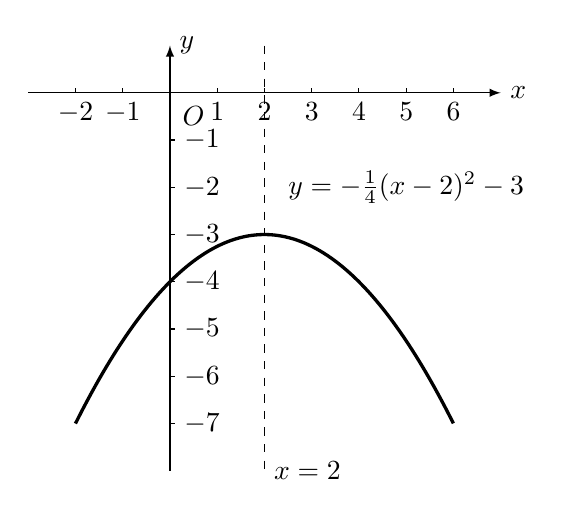
\begin{tikzpicture}[>=latex, scale=.6]
\draw[->] (-3,0)--(7,0)node[right]{$x$};
\draw[->] (0,-8)--(0,1)node[right]{$y$};
\foreach \x in {-2,-1,1,2,...,6}
{
    \draw (\x,0)node[below]{$\x$}--(\x,.1);
}
\foreach \y in {-1,-2,...,-7}
{
    \draw (0,\y)--(.1,\y)node[right]{$\y$};
}
\node at (.5,-.5){$O$};
\draw [domain=-2:6, samples=100, very thick]plot(\x, {-.25*(\x-2)*(\x-2)-3});
\draw[dashed](2,1)--(2,-8)node[right]{$x=2$};
\node at (5,-2){$y=-\frac{1}{4}(x-2)^2-3$};
\end{tikzpicture}
    \caption{}
\end{figure}
\end{solution}


\begin{example}
    平移抛物线$y=ax^2$使顶点在$(2,4)$且$y$截距等于$-8$。
\end{example}

\begin{solution}
    平移抛物线$y=ax^2$使顶点在$(2,4)$, 因此新抛物线的方程是:
   \[ y=a(x-2)^2+4\]
    又$y$截距等于$-8$, 即抛物线通过$(0,-8)$点,因此,
\[\begin{split}
    -8&=a(0-2)^2+4\\
4a&=-12\\
a&=-3
\end{split}\]
所求抛物线方程是 $y=-3(x-2)^2+4$。
\end{solution}

\subsubsection{函数$y=ax^2+bx+c$的图象}
现在我们来研究函数$y=ax^2+bx+c$的图象。
因为
\[\begin{split}
ax^2+bx+c&=a\left(x^2+\frac{b}{a}x\right)+c\\
&=a\left[x^2+\frac{b}{a}x+\left(\frac{b}{2a}\right)^2\right]+c-\frac{b^2}{4a}\\
&=a\left(x+\frac{b}{2a}\right)^2+\frac{4ac-b^2}{4a}
\end{split}\]    
所以函数$y=ax^2+bx+c$可以化成$y=a(x+m)^2+k$的形式,这里$m=\frac{b}{2a}$, $k=\frac{4ac-b^2}{4a}$。

由此可知,函数$y=ax^2+bx+c$的图象和函数$y=ax^2$的
图象完全相同,只是位置不同,它们都是抛物线。

抛物线$y=ax^2+bx+c$, 对称轴方程是
$x=-\frac{b}{2a}$,
顶点坐标是$\left(-\frac{b}{2a},\frac{4ac-b^2}{4a}\right)$。
\begin{itemize}
    \item 当$a>0$时,二次函数$y=ax^2+bx+c$开口向上,在
$x=-\frac{b}{2a}$处取得$y_{\min}=\frac{4ac-b^2}{4a}$;
\item 当$a<0$时,函数开口向下,在$x=-\frac{b}{2a}$处取得$y_{\max}=\frac{4ac-b^2}{4a}$。
\end{itemize}

\begin{example}
    指出下面抛物线的开口
方向,顶点坐标和对称轴方程,
并画出图象:
\begin{multicols}{2}
\begin{enumerate}
    \item $y=2x^2+8x+5$
    \item $y=-x^2+2x+1$
\end{enumerate}
\end{multicols}
\end{example}

\begin{solution}
\begin{enumerate}
    \item 配方:
\[\begin{split}
    y=2x^2+8x+5&=2(x^2+4x)+5\\
    &=2(x^2+4x+4)+5-8\\
    &=2(x+2)^2-3
\end{split}\]

性质:$\because\quad a=2>0$

$\therefore\quad $
抛物线开口向上,顶点坐标是$(-2,-3)$, 对称轴方程是$x=-2$。

作图象:
\begin{center}
\begin{tabular}{c|ccccccccccc}
\hline
$x$&$\cdots$& $-4$ &  $-3\tfrac{1}{2}$ & $-3$ &  $-2\tfrac{1}{2}$ & $-2$ &  $-1\tfrac{1}{2}$ &  $-1$ &  $-\tfrac{1}{2}$ &  0 &$\cdots$\\
\hline
$y$&$\cdots$ & $5$& $1\tfrac{1}{2}$ &  $-1$ &  $-2\tfrac{1}{2}$ &  $-3$ &  $-2\tfrac{1}{2}$ &  $-1$ &  $1\tfrac{1}{2}$ &  $5$ &  $\cdots$ \\
\hline
\end{tabular}
\end{center}  
图象如图5.13。

\item 配方:
\[\begin{split}
    y=-x^2+2x+1&=-(x^2-2x-1)\\
    &=-(x^2-2x)+1\\
    &=-(x^2-2x+1)+2\\
&=-(x-1)^2+2
\end{split}\]

性质:$\because\quad a=-1<0$

$\therefore\quad $
抛物线开口向下,顶点坐标是$(1,2)$, 对称轴方程是$x=1$。

作图象:
\begin{center}
\begin{tabular}{c|ccccccccc}
\hline
$x$&$\cdots$& $-2$ &  $-1$ & 0 & 1 & 2 &  3 &  4 &$\cdots$\\
\hline
$y$&$\cdots$ & $-7$& $-2$ &  1 & 2 & 1 &  $-2$ &  $-7$  &  $\cdots$ \\
\hline
\end{tabular}
\end{center}  
图象如图5.14。

\begin{figure}[htp]\centering
    \begin{minipage}[t]{0.48\textwidth}
    \centering
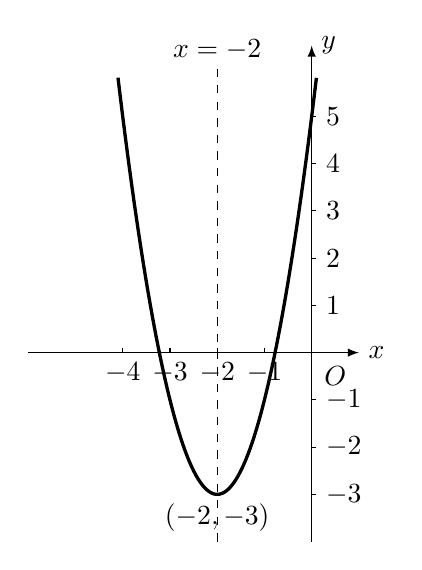
\begin{tikzpicture}[>=latex, scale=.6]
 \draw[->] (-6,0)--(1,0)node[right]{$x$};
\draw[->] (0,-4)--(0,6.5)node[right]{$y$};
\foreach \x in {-4,-3,...,-1}
{
    \draw (\x,0)node[below]{$\x$}--(\x,.1);
}
\foreach \y in {-1,-2,-3,1,2,...,5}
{
    \draw (0,\y)--(.1,\y)node[right]{$\y$};
}
\node at (.5,-.5){$O$};   
\draw[dashed] (-2,-4)--(-2,6)node[above]{$x=-2$};
\node at (-2,-3)[below]{$(-2,-3)$};
\draw [domain=-4.1:0.1, samples=100, very thick]plot(\x, {2*(\x+2)*(\x+2)-3});
    \end{tikzpicture}
    \caption{}
    \end{minipage}
    \begin{minipage}[t]{0.48\textwidth}
    \centering
    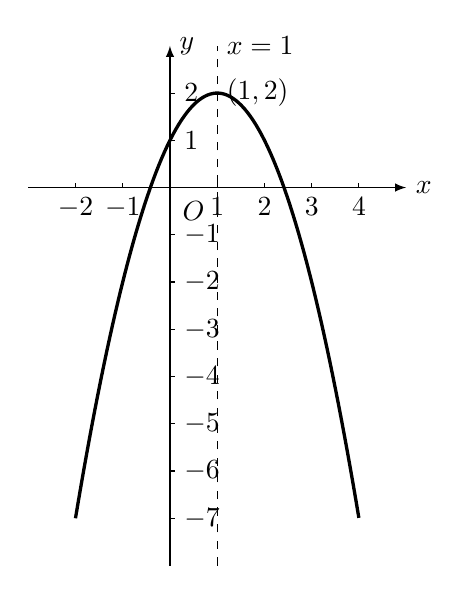
\begin{tikzpicture}[>=latex, scale=.6]
 \draw[->] (-3,0)--(5,0)node[right]{$x$};
\draw[->] (0,-8)--(0,3)node[right]{$y$};
\foreach \x in {-2,-1,1,2,3,4}
{
    \draw (\x,0)node[below]{$\x$}--(\x,.1);
}
\foreach \y in {-1,-2,...,-7,1,2}
{
    \draw (0,\y)--(.1,\y)node[right]{$\y$};
}
\node at (.5,-.5){$O$};          
\draw[dashed] (1,-8)--(1,3)node[right]{$x=1$};
\draw [domain=-2:4, samples=100, very thick]plot(\x, {-(\x-1)*(\x-1)+2});
\node at (1,2)[right]{$(1,2)$};
    \end{tikzpicture}
    \caption{}
    \end{minipage}
    \end{figure}

\end{enumerate}
\end{solution}


\begin{example}
\begin{enumerate}
    \item $k$为何值时,抛物线$y=x^2+2kx+1$的顶点在直线$y=x$上?
    \item 说明上述情况下的抛物线是由怎样的抛物线作怎样的平移得到的。
\end{enumerate}
\end{example}

\begin{solution}
\begin{equation}
    y=x^2+2kx+1=(x+k)^2+1-k^2
\end{equation}
抛物线(5.5)的顶点坐标是$(-k,1-k)$. 顶点在直线$y=x$上
的充要条件是:
\[1-k2=-k\quad \Rightarrow\quad k^2-k-1=0\]
$\therefore\quad k=\frac{1\pm\sqrt{5}}{2}$

因此,当$k=\frac{1+\sqrt{5}}{2}$或$k=\frac{1-\sqrt{5}}{2}$时,抛物线(5.5)的顶点在直
线$y=x$上,这时抛物线方程是:
\begin{equation}
y=\left(x+\frac{1+\sqrt{5}}{2}\right)^2-\frac{1+\sqrt{5}}{2}
\end{equation}
和
\begin{equation}
    \begin{split}
 y&=\left(x+\frac{1-\sqrt{5}}{2}\right)^2-\frac{1-\sqrt{5}}{2}\\
&=\left(x-\frac{\sqrt{5}-1}{2}\right)+\frac{\sqrt{5}-1}{2}
    \end{split}
\end{equation}  

抛物线(5.6)是由抛物线$y=x^2$向左移$\frac{1+\sqrt{5}}{2}$个
单位再向下移$\frac{1+\sqrt{5}}{2}$个单位得来;抛物线(5.7)是由抛物线$y=x^2$向右移
$\frac{\sqrt{5}-1}{2}$个单位再向上移$\frac{\sqrt{5}-1}{2}$个单位
得来。
\end{solution}

\section*{习题5.1}
\addcontentsline{toc}{subsection}{习题5.1}

\begin{enumerate}
    \item 把下列各图象画在同一坐标系里进行比较:
\begin{enumerate}
    \item $y=x,\qquad  y=x+2,\qquad  y=x^2-2$
    \item $y=-x^2,\qquad y=-x^2+2,\qquad y=-x^2-2$
\end{enumerate}

    \item 把下列各图象画在同一坐标系里进行比较:
  \[  y=x^2,\quad     y=(x-1)^2,\quad    y=(x-2)^2,\quad     y=(x-3)^2\]
 \[   y=(x+1)^2,\quad     y=(x+2)^2,\quad     y=(x+3)^2\]
    \item 已知函数$y=2(x-3)^2$, 不作出图象而说出:
\begin{enumerate}
\item 图象的顶点,对称轴方程,开口方向;
\item 函数有没有极大值或极小值?这些值是多少?$x$等
    于什么值时,函数有这些值?
    \item $x$在什么区间时函数是递减的,递增的?
    \item $x$取什么值时函数等于零?
    \item 图象和$y$轴的交点的坐标。
\end{enumerate}

    \item 照上题那样研究$y=-3(x+5)^2$。
    \item 求把抛物线$y=2x^2$向左平移3个单位,再向上平移5个
    单位后的抛物线方程。
    \item 求把抛物线$y=\frac{1}{2}x^2$向右平移5个单位,再向下平移3个
    单位后的抛物线方程。
    \item 将抛物线$y=ax^2$向左平移2个单位后,再向上平移3个单
    位且知这个抛物线与$x$轴的一个交点的坐标是$(2,0)$。
    求这个抛物线方程和它与$x$轴的另一个交点的坐标。
    \item 求下列各函数的图象,并指出所求抛物线的开口方向,
    对称轴方程,顶点坐标,又当$x$为何值,二次函数取得
    什么极值:
\begin{multicols}{2}
    \begin{enumerate}
        \item $y=x^2+6x-3$
        \item $y=2x^2-5x+2$
        \item $y=5-x-x^2$
        \item $y=6+12x-3x^2$
        \item $y=-2x^2-5x+7$
        \item $y=3x^2+2x$
        \item $y=\frac{5}{2}x-2-3x^2$
        \item $y=\frac{1}{2}x^2+3x+\frac{5}{2}$
    \end{enumerate}
\end{multicols}

\item 处于静止状态的物体从40米的高处下落,计算$t$秒后物
体离地面的高度$h$米的公式是$h=40-5t^2$
\begin{enumerate}
    \item 经过两秒钟物体离地面的高度是多少?
    \item 经过多少时间物体落到地面?
    \item 求出时间$t$的取值范围。
    \item 作出$h$和$t$之间的函数关系的图象。
\end{enumerate}

\item 一石子从井口落下,经过7秒后听到碰击井底声,如果
石子下降距离$s$(米)与经过的时间$t$(秒)的关系是$s=5t^2$,
又声音在空气中的平均速度是每秒340米,求井深。
\end{enumerate}

\section{和二次函数有关的课题}
\subsection{根据已知条件确定二次函数}
在上一节里我们研究了二次函数的图象和它的性质,现
在我们进一步来研究,如何根据二次函数满足的条件来确定
这个二次函数的问题,下面我们来看几个例题:


\begin{example}
    已经知道函数$y=f(x)$是一个二次函数,并且知
道它的图象通过$A(0,1)$, $B(1,3)$, $C(-1,1)$三点,写出
这个二次函数。
\end{example}

\begin{solution}
二次函数的一般形式是
\begin{equation}
    y=ax^2+bx+c
\end{equation}
要确定这个函数,必须知道二次三项式里三个系数$a,b,c$的
值。由函数图象的定义知道,图象上的点的坐标必适合函数
关系式,现在已知$A,B,C$三点在图象上,故它们的坐标必适
合关系式(5.8), 因此可以列出关于$a,b,c$的三元一次方程
组:
\[\begin{cases}
    1=a\cdot 0^2+b\cdot 0+c\\
3=a\cdot 1^2+b\cdot 1+c\\
1=a(-1)^2+b(-1)+c
\end{cases}\]
即:
\begin{equation}
    \begin{cases}
        c=1\\
a+b+c=3\\
a-b+c=1
    \end{cases}
\end{equation}
解方程组(5.9)得
\[a=1,\qquad b=1,\qquad c=1\]
所求的二次函数是
$y=x^2+x+1$。
\end{solution}
    

\begin{example}
    已知二次函数的图象与$x$轴交于$(-2,0)$和$(1,
0)$两点,又通过点$(3,-5)$, 求这个二次函数的表达式、它
的极值点和极值。
\end{example}

\begin{solution}
二次函数$f(x)=ax^2+bx+c$的图象与$x$轴交于两点
$(-2,0)$, $(1,0)$的意思,是说函数值$f(-2)=0$和$f(1)=
0$。根据余式定理的推论2, $(x+2)(x-1)$必能整除$f(x)=
ax^2+bx+c$. 因此这个二次函数表达式可以写成:
\[f(x)=a(x+2)(x-1)\]
又它的图象通过点$(3,-5)$, 即$f(3)=-5$, 将$x=3$和$x=-5$
代入上式得
\[-5=a(3+2)(3-1)\]
$\therefore\quad a=-\frac{1}{2}$。

因此所求二次函数表达式是:
\begin{equation}
    \begin{split}
        f(x)&=-\frac{1}{2}(x+2)(x-1)\\
        &=-\frac{1}{2}(x^2+x-2)\\
        &=-\frac{1}{2}x^2-\frac{1}{2}+1
    \end{split}
\end{equation}

因为抛物线顶点的横坐标等于对称轴与$x$轴的交点的横
坐标,设顶点横坐标是$x_0$, 于是在$x$轴上有
    \[x_0-(-2)=1-x_0\]
    即:$x_0=\frac{(-2)+1}{2}=-\frac{1}{2}$(图5.15)
代入(5.10)得顶点纵坐标:
\[y_0=f\left(-\frac{1}{2}\right)=-\frac{1}{2}\left(\frac{1}{4}-\frac{1}{2}-2\right)=\frac{9}{8}\]

$\because\quad a=-\frac{1}{2}<0$

$\therefore\quad $在$x_0=-\frac{1}{2}$处$y_{\max}=\frac{9}{8}$。

\begin{figure}[htp]
    \centering
    \begin{tikzpicture}[>=latex]
 \draw[->] (-3,0)--(3,0)node[right]{$x$};
\draw[->] (0,-3)--(0,2)node[right]{$y$};
\draw[dashed] (-.5,-3)--(-.5,2);
\draw [domain=-3:2, samples=100, thick]plot(\x, {-0.5*(\x*\x+\x-2)});
\foreach \x in {-2,1}
{
    \node at (\x, 0)[below]{$\x$};
}
\node at (-.5,0)[below]{$x_0$};
\node at (.25,-.25){$O$};       
    \end{tikzpicture}

    \caption{}
\end{figure}
\end{solution}

\begin{rmk}
    我们在求函数的极值点与极值时没有应用前面给
出的公式,而是借助于二次函
数的图象的顶点在对称轴上。
\end{rmk}

结合图象来研究二次函数
的性质是解决问题的一个途径。

\begin{example}
    已知函数$y=ax^2+bx+c$的图象是以点$(2,3)$为
顶点的抛物线,并且这图象通过$(3,1)$, 写出这个函数。
\end{example}

\begin{solution}
\textbf{解法1:} 抛物线$y=ax^2+bx+c$的顶点坐标是:$\left(-\frac{b}{2a},\frac{4ac-b^2}{4a}\right)$,根据已知条件得:
\begin{align}
    -\frac{b}{2a}&=2\\
\frac{4ac-b^2}{4a}&=3
\end{align}
另外根据抛物线通过点$(3,1)$, 又可得到一个方程:
\begin{equation}
    1=9a+3b+c
\end{equation}
把(5.11), (5.12), (5.13)联立,就可得到关于$a,b,c$的方程组:
\begin{equation}
    \begin{cases}
        -\frac{b}{2a}&=2\\
\frac{4ac-b^2}{4a}&=3\\
9a+3b+c=1
    \end{cases}
\end{equation}
解方程组(5.14), 得
\[a=-2,\qquad b=8,\qquad c=-5\]
所求的二次函数是$y=-2x^3+8x-5$。

\textbf{解法2:} 以点$(m,k)$为顶点的抛物线方程是$y=a(x-m)^2+k$。
这样根据已知条件,就可以写出所求的二次函数是
\begin{equation}
    y=a(x-2)^2+3
\end{equation}
因为点$(3,1)$在图象上,所以把$x=3$, $y=1$代入(5.15)得到
\[1=a(3-2)^2+3\]
由此得$a=-2$. 把它代入(5.15)就得
\[y=-2(x-2)^2+3=-2x^2+8x-5\]
故所求二次函数是$y=-2x^2+8x-5$。

解法2要比解法1方便些。
\end{solution}

由上面讨论可知,要确定一个二次函数需要三个独立条
件去确定系数$a,b,c$, 若条件中有顶点坐标(如例5.13),那么
这个顶点坐标算两个独立条件,这是因为顶点已知的话,所
求抛物线的位置已经确定,所剩就是确定抛物线的开口情况
(即系数$a$),故只要再有一个条件就可确定了。

\begin{ex}
\begin{enumerate}
\item 求经过$A(0,1)$, $B(-1,1)$, $C(1,-1)$三点,且对称
    轴平行于$y$轴的抛物线,并求其顶点坐标和对称轴。
    \item 设有函数$y=x^2+px+q$, 按照下列条件,求$p$和$q$的值。
    \begin{enumerate}
 \item 在$x=2$时,$y=12$, 在$x=-3$时,$y=2$;
    \item 在$x=5$时,函数有极小值$-2$;
    \item 函数的图象和$x$轴的交点的坐标是$(-4,0)$和$(-1,
    0)$.
    \end{enumerate}
   
    \item 设有二次函数$y=ax^2+bx+c$, 按照下列条件,求出$a,b,
    c$的值,然后写出这个二次函数:
    \begin{center}
        \begin{tabular}{c|ccc}
            \hline
$x$&1&2&3\\
            \hline
$y$&0&0&4\\
            \hline
        \end{tabular}
    \end{center}
    函数的图象是以点$A(-1,-8)$为顶点的抛物线,
   并且和$y$轴交于点$B(0,-6)$。

    \item 抛物线$y=x^2+2ax+b$经过点$(2,4)$, 并且其顶点在
    $y-2x-1=0$上,求$a,b$。
    \item 若$f(x)$是二次函数,当$x=\frac{1}{2}$时有极大值25,又方程
    $f(x)=0$的二根平方和等于13, 求$f(x)$。
\end{enumerate} 
\end{ex}

\subsection{二次函数极值}
根据实数的平方不小于零,容易求得二次函数的极值如
下:
\[y=ax^2+bx+c=a\left(x+\frac{b}{2a}\right)^2+\frac{4ac-b^2}{4a}\]
\begin{enumerate}
    \item 如果$a>0$, 那么$a\left(x+\frac{b}{2a}\right)^2\ge 0$
\[y=a\left(x+\frac{b}{2a}\right)^2+\frac{4ac-b^2}{4a}\ge \frac{4ac-b^2}{4a}\]
即当$x=-\frac{b}{2a}$时,函数有极小值,$y_{\min}=\frac{4ac-b^2}{4a}$

\item 如果$a<0$, 那么$a\left(x+\frac{b}{2a} \right)^2\le 0$
\[y=a\left(x+\frac{b}{2a}\right)^2+\frac{4ac-b^2}{4a}\le \frac{4ac-b^2}{4a}\]
即当$x=-\frac{b}{2a}$时,函数有极大值,$y_{\max}=\frac{4ac-b^2}{4a}$
\end{enumerate}

求二次函数的极值有着许多实际的应用,下面我们举几
个例子。

\begin{example}
    某工厂为了存放材料,需要围一个周长为160米
的矩形场地,问矩形的长和宽各取多少米,才能使存放场地
的面积最大?
\end{example}

\begin{solution}
    设一边为$x$m,则另一边长为$(80-x)$m,如果$y{\rm m}^2$
是矩形的面积,则
\[\begin{split}
    y=x(80-x)&=-x2+80x,\qquad (0<x<80)\\
    &=-(x^2-80x+1600-1600)\\
    &=-(x-40)^2+1600
\end{split}\]
因此,当边长是40m的正
方形时,有最大面积1600${\rm m}^2$。
\end{solution}

\begin{example}
    窗的形状是矩形上
面加一个半圆,它的周长等于
6米,要使窗能透过最多的光
线,它的尺寸应该怎样设计?
\end{example}

\begin{solution}
设半圆的半径是$x$米(图5.16),那么半圆的长就是
$\pi x$米,矩形的底$BC$就是$2x$米,而矩形的高$AB$和$CD$就是
$\frac{6-\pi x-2x}{2}$米。

\begin{figure}[htp]
    \centering
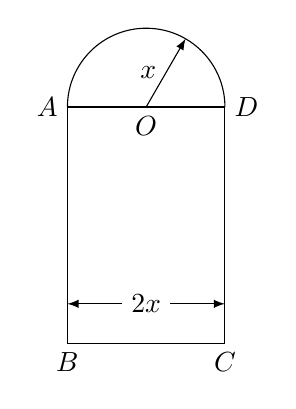
\begin{tikzpicture}[>=latex]
\draw (0,0) rectangle (2,3) node [right]{$D$};
\node at (0,0)[below]{$B$};
\node at (2,0)[below]{$C$};
\node at (0,3)[left]{$A$};
\node at (1,3)[below]{$O$};
\draw (0,3) arc (180:0:1);
\draw[->] (1,3)--node[left]{$x$} +(60:1) ;
\draw [<->](0,.5)--node[fill=white]{$2x$}(2,.5);
\end{tikzpicture}
    \caption{}
\end{figure}

设图形的总面积是$y$平方米,那么在开区间$\left(0,\frac{6}{\pi+2}\right)$上,
\[y=\frac{6-\pi x-2x}{2}\cdot 2x+\frac{1}{2}\pi x^2\]
就是
\[\begin{split}
    y&=6x-\left(\frac{\pi}{2}+2\right)x^2\\
    &=-\frac{\pi+4}{2}\left[x^2-\frac{12}{\pi+4}x+\left(\frac{6}{\pi+4}\right)^2-\left(\frac{6}{\pi+4}\right)^2\right]\\
    &=-\frac{\pi+4}{2}\left(x-\frac{6}{\pi+4}\right)^2+\frac{18}{\pi+4}
\end{split}\]
由此可知,当$x=\frac{6}{\pi+4}$的时候,$y_{\max}=\frac{18}{\pi+4}$。

所以尺寸应该这样来设计:半圆的半径是$\frac{6}{\pi+4}\approx 0.84$米,或者说矩形的底边长是$\frac{12}{\pi+4}\approx 1.68$米时,窗能透过最
多的光线。
\end{solution}

\begin{example}
    用一块宽为1.2米的长方形铁板弯起两边做一个
水槽,水槽的横截面为底角是$120^{\circ}$的等腰梯形(图5.17),要
使水權的横截面积最大,它的侧面的宽应该是多少?
\end{example}

\begin{figure}[htp]
    \centering
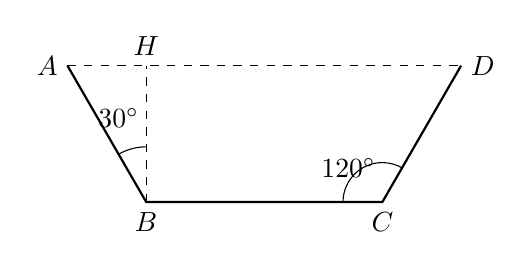
\begin{tikzpicture}
\draw[thick] (120:2)--(0,0)node[below]{$B$}--(3,0)node[below]{$C$}--+(60:2);
\draw[dashed] (-1,1.732)node[left]{$A$}--(4,1.732)node[right]{$D$};
\draw [dashed](0,0)--(0,1.732)node[above]{$H$};
\draw (0,.7) arc (90:120:.7)node[above=6pt]{$30^{\circ}$};
\draw(2.5,0) arc (180:60:.5)node [left=6pt]{$120^{\circ}$};
\end{tikzpicture}   
    \caption{}
\end{figure}


\begin{solution}
    设侧的宽$AB$为$x$米,作$BH\bot AD$, 则
\[\angle ABH=30^{\circ},\qquad AH=x\sin 30^{\circ}=\frac{1}{2}x\]
\[BH=x\cdot \cos 30^{\circ}=\frac{\sqrt{3}}{2}x,\qquad BC=(1.2-2x)\]
\[AD=1.2-2x+2\cdot \frac{x}{2}=1.2-x\]
所以,水槽的横截面面积为:
\[\begin{split}
    S&=\frac{1}{2}\cdot \frac{\sqrt{3}}{2}x(1.2-2x+1.2-x)\\
    &=\frac{\sqrt{3}}{4}x(2.4-3x)\qquad (0<x<0.6)\\
    &=-\frac{3\sqrt{3}}{4}x^2+\frac{3\sqrt{3}}{5}x=-\frac{3\sqrt{3}}{4}\left(x^2-\frac{4}{5}x\right)\\
&=-\frac{3\sqrt{3}}{4}\left(x^2-\frac{4}{5}x+\frac{4}{25}-\frac{4}{25}\right)\\
&=-\frac{3\sqrt{3}}{4}\left(x-\frac{2}{5}\right)^2+\frac{3\sqrt{3}}{25}
\end{split}\]
所以$x=\frac{2}{5}=0.4$(米)时,水槽有最大的横截面面积$\frac{3\sqrt{3}}{25}$(平方米)。
\end{solution}


\begin{example}
    快艇和轮船分别从$A$地和$C$地同时开出,各沿着
    箭头所指方向航行(图5.18),快艇和轮船的速度分别是40公
    里/小时和16公里/小时,已知$AC=145$公里,经过多少时间
    以后,快艇和轮船之间的距离最短(图中$AC\bot CD$)?
\end{example}

\begin{figure}[htp]
    \centering
\begin{tikzpicture}[>=latex, scale=.9]
\draw (0,0)--(8,0)node[right]{$A$};
\draw[->, very thick] (0,0)--(0,-2)node[below]{$D$};
\draw[->, very thick] (8,0)--(3,0)node[above]{$B$};
\draw (0,-2)--(3,0);
\draw (3,0)--(3,-1); \draw (8,0)--(8,-1); 
\draw[<->] (3,-.5)--node[fill=white]{$40t$}(8,-.5);
\draw (-1,0)--(0,0); \draw (-1,-2)--(0,-2);
\draw[<->]  (-.5,0)--node[fill=white]{$16t$}(-.5,-2);
\node at (-.25,.25) {$C$};
\draw(0,0)--(0,1.2); \draw (8,0)--(8,1.2);
\draw[<->] (0,1) --node[fill=white]{$145$公里}  (8,1) ;

\end{tikzpicture}
    \caption{}
\end{figure}

\begin{solution}
    设经过$t$小时以后,快艇的位置在$B$, 轮船的位置在
$D$. 这时
\[\begin{split}
  AB&=40t \text{(公里)}\\
CD&=16t \text{(公里)}\\
BC&=(145-40t) \text{(公里)}\\  
\end{split}\]
根据勾股定理得
\[BD=\sqrt{BC^2+CD^2}=\sqrt{(145-40t)^2+(16t)^2}\]
现在要使$BD$最短,因$(145-40t)^2+(16t)^2>0$

故只需使被开方数$(145-40t)^2+(16t)^2$有最小的值。

令 $y=(145-40t)^2+(16t)^2\qquad \left(0<t<3\frac{5}{8}\right)$
则有:$$y=1856t^2-11600t+21025$$
这个二次函数在
$t=\frac{11600}{3712}=3\frac{1}{8}$(小时)
的时候有极小值。所以,快艇和轮船分别从$A$地和$C$地开出
$3\frac{1}{8}$(小时)的时候,它们间的距离最短。
\end{solution}

有时要在闭区间$[a,b]$上讨论二次函数的最大值或最小
值,这时要把开区间$(a,b)$内的极值和两端点处的函数值作
比较,再确定出最大值或最小值。


\begin{example}    
设$0\le x\le 3$, 讨论$y=x^2-4x+5$的最大值和最小
值。
\end{example}

\begin{solution}    
$$y=(x-2)^2+1$$

当$x=2$时,$y_{\min}=1$;又当$x=0$时,$y=5$;当$x=3$时,$y=2$。

所以当$x=2$时,$y$取最小值
$y_{\min}=1$;当$x=0$时,$y$取最大值$y_{\max}=5$(图5.19)。

\begin{figure}[htp]
    \centering
\begin{tikzpicture}[>=latex,scale=.8]
\draw[->] (-1,0)--(4,0)node[right]{$x$};
\draw[->] (0,-1)--(0,6)node[right]{$y$};
\foreach \x in {1,2,3}
{
    \draw(\x,0)node[below]{$\x$}--(\x,.1);
    \draw(0,\x)node[left]{$\x$}--(.1,\x);
}
\draw(0,4)node[left]{$4$}--(.1,4);
\draw(0,5)node[left]{$5$}--(.1,5);

\draw [domain=0:3, samples=50, very thick]plot(\x, {(\x-2)*(\x-2)+1});
\draw[dashed] (2,-1)--(2,6);
\draw[dashed] (3,0)--(3,2)--(0,2);
\end{tikzpicture}
    \caption{}
\end{figure}
\end{solution}    

\section*{习题5.2}
\addcontentsline{toc}{subsection}{习题5.2}
\begin{enumerate}
    \item 求下列各函数的最大值和最小值,并且求这时的$x$的值:
\begin{multicols}{2}
\begin{enumerate}
    \item $y=x^2-6x+10$
    \item $y=3x^2+6x-2$
    \item $y=5-4x-x^2$
    \item $y=3+2x-2x^2$
\end{enumerate}
\end{multicols}
    \item 求下列各函数的最大值和最小值:
\begin{enumerate}
    \item $y=2x^2+5x+4,\qquad    0\le x\le 1$
    \item $y=x^2-3x+4,\qquad      0\le x\le 1$
    \item $y=x^2-x+1,\qquad      0\le x\le 1$
\end{enumerate}
\item 求证在周长相同的所有矩形中,正方形面积是最大的。
\item 求证在一边长固定,且周长固定的所有三角形中,等腰
三角形面积是最大的。
\item 把宽40厘米的铁皮制成U字形的雨水槽,要使它的断面
积成为最大,深度应为多少?
\item 一农民准备用篱笆围成一面靠墙的矩形,养鸡场共分五
间,每间大小相等,现有可编120米长的篱笆竹料,养
鸡场每间的长宽各是多少米,养鸡场面积最大。
\item 炮弹以初速度$U_0=600$米/秒,仰角$\theta=30^{\circ}$射出时,上升
的高度$h$与相应的水平距离$x$之间的函数关系是:
\[h=-\frac{1}{54000}x^2+\frac{1}{\sqrt{3}}x\]
试求炮弹能达到的最大高度。
\item 设有边长为$a$的等边三角形,要作内接矩形(如图),问如
何作法使这矩形面积最大?
\item 在半径是20厘米的圆内作一内接矩形,这个矩形的面积
最大可以是多少平方厘米?
\item 给了一个正方形$ABCD$(如图)。由它的各顶点量下相等
的线段$Aa,Bb,Cc,Dd$, 并且以直线连结$a,b,c,d$各
点,问$Aa$多长时正方形$abcd$的面积最小?
\item 已知三角形的两边之和为4, 夹角是$60^{\circ}$, 求:最大
面积;最小周长.

\begin{center}
\begin{tikzpicture}[>=latex]
\begin{scope}
    \draw (0,0)--(2,0)--(1,1.732)--(0,0);
\draw[pattern=north east lines] (.5,0) rectangle (1.5,1.732/2);
\node at (1,-1){第8题};
\draw[|<->|](1-.25,1.732+.1)--node[fill=white]{$a$}(0-.25,0+.1);

\end{scope}    
\begin{scope}[xshift=5cm, yshift=1cm]
\draw (0,0) circle (1.5);
\draw (0,0)node[left]{$O$}--node[below]{20cm}(1.5,0)--(120:1.5)--(180:1.5)--(-60:1.5)--(1.5,0);
\node at (0,-2){第9题};
\end{scope}  
\begin{scope}[xshift=8cm]
    \draw (0,0)node[below]{$A$} rectangle(2.1,2.1)node[above]{$C$};
\node at (2.1,0)[below]{$B$}; 
\node at (0,2.1)[above]{$D$}; 

\node at (1.05,-1){第10题};

\draw (0.9,0)node[below]{$a$}--(2.1,.9)node[right]{$b$}--(1.2,2.1)node[above]{$c$}--(0,1.2)node[left]{$d$}--(.9,0); 
\end{scope}  
\end{tikzpicture} 
\end{center}
\end{enumerate}

\subsection{一元二次方程图象解法}
我们来观察二次函数$y=x^2-2x-3=(x-1)^2-4$的图
象(图5.21),这条抛物线交$x$轴于两点:$A(-1,0)$, $B(3,0)$.

这就是说,当$x=-1$或$x=3$时,函数$y=x^2-2x-3$的
值是0, 换句话说,也就是$x=-1$和$x=3$是方程
$x^2-2x-3=0$
的两个根,这个例子告诉我们,二次方程
$ax^2+bx+c=0$
的求根问题可归结为二次函数$y=ax^2+bx+c$对于怎样的$x$取
值为零的问题,这样的$x$称作二次函数的零点,因此二次方程
$ax^2+bx+c=0$的(实)根就等同于二次函数$y=ax^2+bx+c$的零点,这样我们就可用图象来解二次方程,如

\begin{figure}[htp]\centering
    \begin{minipage}[t]{0.48\textwidth}
    \centering
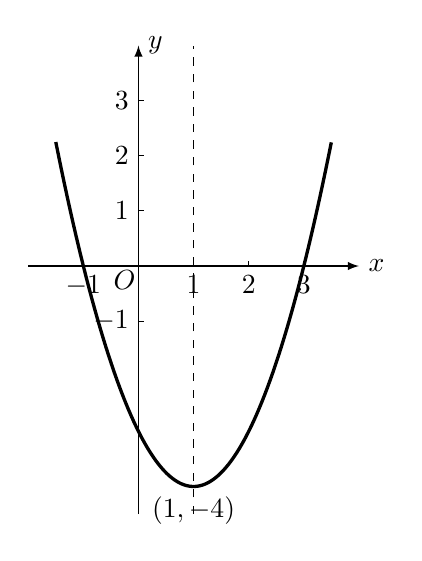
\begin{tikzpicture}[>=latex, scale=.7]
\draw[->] (-2,0)--(4,0)node[right]{$x$};
\draw[->] (0,-4.5)--(0,4)node[right]{$y$};
\foreach \x in {1,2,3,-1}
{
    \draw(\x,0)node[below]{$\x$}--(\x,.1);
    \draw(0,\x)node[left]{$\x$}--(.1,\x);
}       

\draw[dashed] (1,-4.5)--(1,4);
\draw [domain=-1.5:3.5, samples=100, very thick] plot(\x, {(\x-1)*(\x-1)-4});
\node at (1,-4)[below]{$(1,-4)$};
\node at (-.25,-.25){$O$};
    \end{tikzpicture}
    \caption{}
    \end{minipage}
    \begin{minipage}[t]{0.48\textwidth}
    \centering
    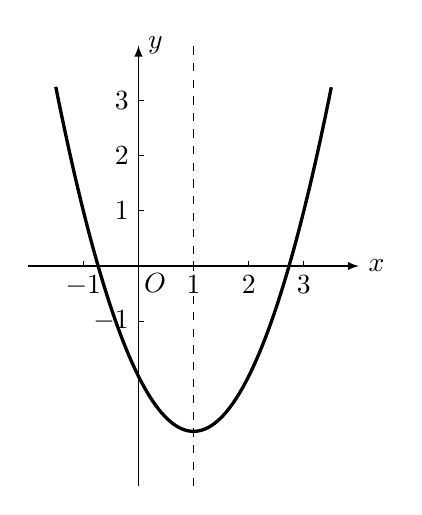
\begin{tikzpicture}[>=latex, scale=.7]
\draw[->] (-2,0)--(4,0)node[right]{$x$};
\draw[->] (0,-4)--(0,4)node[right]{$y$};
\foreach \x in {1,2,3,-1}
{
    \draw(\x,0)node[below]{$\x$}--(\x,.1);
    \draw(0,\x)node[left]{$\x$}--(.1,\x);
}          

\draw[dashed] (1,-4)--(1,4);
\draw [domain=-1.5:3.5, samples=100, very thick] plot(\x, {(\x-1)*(\x-1)-3});
\node at (.3,-.3){$O$};
    \end{tikzpicture}
    \caption{}
    \end{minipage}
    \end{figure}


\begin{example}
    用图象法解一元二次方程
$x^2-2x-2=0$。
\end{example}

\begin{solution}
    先作出函数$y=x^2-2x-2=(x-1)^2-3$的图象(图
5.21),从图中读出二次函数零点:$x_1\approx-0.7$; $x_2\approx 2.7$, 这
就是二次方程$x^2-2x-2=0$的两个近似实根。
\end{solution}

从函数图象的观点看来,二次函数$y=ax^2+bx+c$的零
点,就是它的图象与$x$轴的交点的横坐标,因此二次方程
$ax^2+bx+c=0$能否有实数解,或者有一个(实)重根,或者
有两个不同的(实)根,实际上就等于抛物线$y=ax^2+bx+c$是
否与$x$轴相交,或者与$x$轴相切于一点;或者与$x$轴相交于两
个不同的点(这两个点必对称地位于抛物线对称轴的左、右两
侧)。

当$a>0$时,抛物线$y=ax^2+bx+c$是开口向上的,并且
其顶点是它的最低点,因此二次方程$ax^2+bx+c=0$能否有
解,有一解或二解,完全取决于抛物线$y=ax^2+bx+c$的顶
点位于$x$轴的上方,位于$x$轴上,或位于$x$轴的下方。

抛物线$y=ax^2+bx+c$的顶点坐标是$\left(-\frac{b}{2a},\frac{4ac-b^2}{4a}\right)$
由于$a>0$, 因此抛物线的顶点位于$x$轴的上方,位于$x$轴上,
或者位于$x$轴的下方,分别取决于$b^2-4ac<0$, $b^2-4ac=0$,
或$b^2-4ac>0$ (图5.22),以前我们曾谈过:二次方程$ax^2+bx+c=0$能否有解,取决于判别式$b^2-4ac$的符号,现在我们又
可以看到,抛物线$y=ax^2+bx+c$能否与$x$轴有交点,也取决
于判别式$b^2-4ac$的符号。

当$a<0$时,情况与上面相同,我们留给同学去考虑。

\begin{figure}[htp]
    \centering
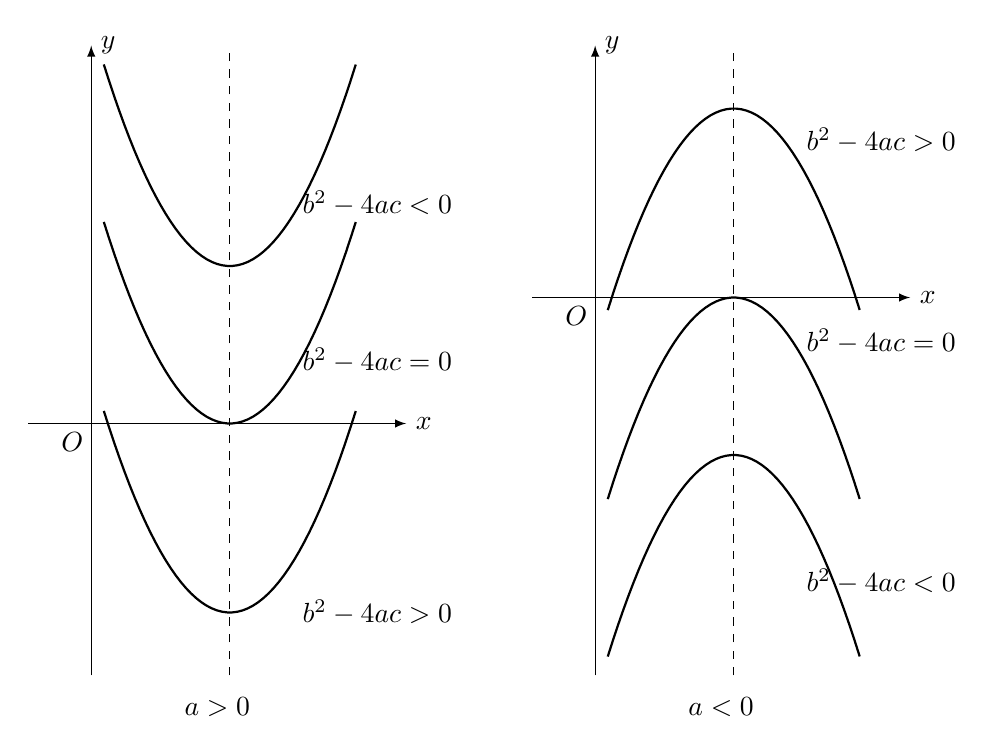
\begin{tikzpicture}[>=latex, scale=.8]
\begin{scope}
    \draw[->] (-1,0)--(5,0)node[right]{$x$};
    \draw[->] (0,-4)--(0,6)node[right]{$y$};
    \draw[domain=.2:4.2, samples=50, thick]plot(\x, {(\x-2.2)*(\x-2.2)*.8});
    \draw[domain=.2:4.2, samples=50, thick]plot(\x, {(\x-2.2)*(\x-2.2)*.8+2.5});
    \draw[domain=.2:4.2, samples=50, thick]plot(\x, {(\x-2.2)*(\x-2.2)*.8-3});
    \draw[dashed] (2.2,-4)--(2.2,6);
    \node at (-.3,-.3){$O$};
    \node at (2,-4.5){$a>0$};
\node at (3.2,-3)[right]{$b^2-4ac>0$};
\node at (3.2,1)[right]{$b^2-4ac=0$};
\node at (3.2,3.5)[right]{$b^2-4ac<0$};
\end{scope}

\begin{scope}[xshift=8cm, yshift=2cm]
    \draw[->] (-1,0)--(5,0)node[right]{$x$};
    \draw[->] (0,-6)--(0,4)node[right]{$y$};
    \draw[domain=.2:4.2, samples=50, thick]plot(\x, {-(\x-2.2)*(\x-2.2)*.8});
    \draw[domain=.2:4.2, samples=50, thick]plot(\x, {-(\x-2.2)*(\x-2.2)*.8-2.5});
    \draw[domain=.2:4.2, samples=50, thick]plot(\x, {-(\x-2.2)*(\x-2.2)*.8+3});
    \draw[dashed] (2.2,-6)--(2.2,4);
    \node at (-.3,-.3){$O$};
    \node at (2,-6.5){$a<0$};
    \node at (3.2,-4.5)[right]{$b^2-4ac<0$};
    \node at (3.2,-.7)[right]{$b^2-4ac=0$};
    \node at (3.2,2.5)[right]{$b^2-4ac>0$};
\end{scope}
\end{tikzpicture}
    \caption{}
\end{figure}

前面考虑二次方程$ax^2+bx+c=0$的根为二次函数$y=
ax^2+bx+c$的图象与$x$轴的交点的横坐标,我们也可用另外一种观点来考虑。由于
$ax^2+bx+c=0$与$ax^2=-bx-c$
的解是一样的,故我们可以考虑抛物线
$y=ax^2$与直线$y=-bx-c$的交点。

为此,在同一坐标系里,把抛物线和直线画出来,如果直
线与抛物线有交点(至多两个)那么交点的横坐标就是二次方
程的根。这是因为,如果交点是$(x_1,y_1)$, 那么必有$y_1=ax_1^2$和
$y_1=-bx_1-c$, 从而有$ax_1^2=-bx_1-c$, 即$ax_1^2+bx_1+c=0$。
如果没有交点,则二次方程
没有解。当我们使用函数图象求解二次方程近似根时,
这种方法是比较方便的,因
为$y=ax^2$与$y=-bx-c$都比
较容易描绘,如果我们还是
以例5.19的二次方程$x^2-2x-2=0$为例,如图5.23,
求出近似根$x_1\approx -0.7$,$x_2\approx 2.7$。

\begin{figure}[htp]
    \centering
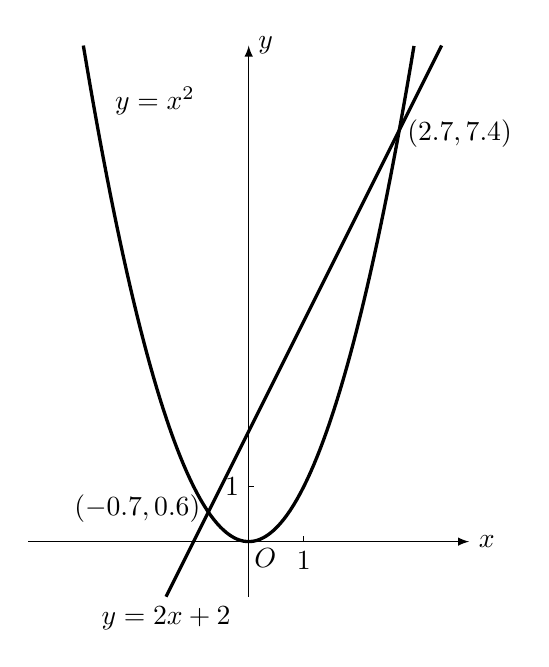
\begin{tikzpicture}[>=latex, scale=.7]
\draw[->] (-4,0)--(4,0)node[right]{$x$};
\draw[->] (0,-1)--(0,9)node[right]{$y$};
\foreach \x in {1}
{
    \draw(\x,0)node[below]{$\x$}--(\x,.1);
    \draw(0,\x)node[left]{$\x$}--(.1,\x);
}          

\draw [domain=-3:3, samples=100, very thick] plot(\x, {\x*\x});
\draw [domain=-1.5:3.5, samples=10, very thick] plot(\x, {2*\x+2});
\node at (-1.5,-1)[below]{$y=2x+2$};
\node at (-1.7,8){$y=x^2$};
\node at (2.7,7.4)[right]{$(2.7,7.4)$};
\node at (-.7,.6)[left]{$(-0.7,0.6)$};
\node at (.3,-.3){$O$};
    \end{tikzpicture}
    \caption{}
\end{figure}




\begin{example}
    
\end{example}

\begin{solution}
    
\end{solution}


\begin{example}
    
\end{example}

\begin{solution}
    
\end{solution}

\begin{example}
    
\end{example}

\begin{solution}
    
\end{solution}


\begin{example}
    
\end{example}

\begin{solution}
    
\end{solution}

\begin{example}
    
\end{example}

\begin{solution}
    
\end{solution}








\begin{example}
    
\end{example}

\begin{solution}
    
\end{solution}


\begin{example}
    
\end{example}

\begin{solution}
    
\end{solution}


\begin{example}
    
\end{example}

\begin{solution}
    
\end{solution}

\begin{example}
    
\end{example}

\begin{solution}
    
\end{solution}


\begin{example}
    
\end{example}

\begin{solution}
    
\end{solution}

\begin{example}
    
\end{example}

\begin{solution}
    
\end{solution}















\begin{ex}
\begin{enumerate}
    \item 证明函数$y=x^3+x$处处递增。
    \item 求下面函数的极大值和极小值:
\begin{enumerate}
    \item $y=2x^3-9x^2+12x+5$
    \item $y=4x^3-6x^2-9x+1$
\end{enumerate}
    \item 求内接于半径为$R$的球中的直圆柱的最大体积。
    \item 某自来水厂设计一座圆柱形自来水塔,它的全面积合计
    为$150\pi$平方米,要使这座水塔有最大的容量,应该怎样
    定出水塔的高和底面圆的半径,才能达到最大容量的要
    求,并算出水塔的容量。
\end{enumerate}
\end{ex}

\section*{复习题五}
\addcontentsline{toc}{section}{复习题五}
\begin{enumerate}
    \item 指出下列函数图象的顶点,对称轴和开口方向:
\begin{multicols}{2}
\begin{enumerate}
    \item $y=2x^2-16x+32$
    \item $y=4x^2+12x-7$
    \item $y=-2x^2-4x+6$
    \item $y=1+4x-x^2$
    \item $y=(1-x)^2+2$
    \item $y=2(x-2)(x+3)$
\end{enumerate}
\end{multicols}
   \item  已知下列函数:
\begin{multicols}{2}
\begin{enumerate}
\item $y=x^2+4x-5$
\item $y=x^2-4x+1$
\item $y=6-4x-2x^2$
\item $y=-\frac{1}{4}x^2+x-1$
\item $y=(x-2)(x-3)$
\item $y=(2x+1)(3-x)$
\end{enumerate}
\end{multicols}
   问: \begin{enumerate}
       \item $x$取什么值时,$y=0$? $y>0$? $y<0$?
       \item 当$x$取什么值时,函数是增函数,减函数,并求出
   极值点和极值。
   \item 画出它们的图象。
   \end{enumerate}
\item 把24, 27, 34, 37各分成两个正整数,使它们的乘积最
大。
\item 抛物线$y=-\frac{1}{2}x^2+\frac{9}{2}x-6$, 当$x$的取值在什么范围
内,位于直线$y=\frac{1}{2}x$的下方。
\item 平移抛物线$y=\frac{1}{2}x^2$, 使顶点到$P(t,t^2)$点,并通过$A(2,
4)$点,求平移后的抛物线方程。


\item 求函数$y=\frac{1}{\sqrt{x^2+4x+7}}$的定义域和值域。

\item 通过作函数$y=|x^2+2x-3|$的图象,写出函数的递增
区间和递减区间,并给出函数的极值点和极值。
\item 按照自变量$x$可取值的范围,画出函数$y=\sqrt{-x^2+3x-2}$
的图象,并求最大值和最小值。
\item 已知二次函数$y=x^2+px+q$的图象和$x$轴交于$(1,0)$和
$(-6,0)$两点,求$p,q$的值。
\item 已知二次函数$y=ax^2+bx+c$, 按照下面的条件确定$a,
b,c$的值。
\begin{enumerate}
\item $x=6$时,$y=0$; $x=4$时,函数有极小值$-8$;
\item $x=\frac{1}{2}$时,函数有极大值25; $x=0$时,$y=24$;
\item 顶点是$(6,-12)$, 开口向上,且和$x$轴的一个交点是
$(8,0)$;
\item 顶点是$(2,-7)$, 开口向下,且和$y$轴有一个交点
$(0,-15)$。
\end{enumerate}

\item  $m$为何值使二次方程$x^2+(m-2)x-(m+3)=0$的二
根平方和有最小值。
\item 求$m$的范围,使方程$x^2+(m-2)x-(m+3)=0$的二根
都是正数。
\item  求$p$的范围,使方程$px^2-x+p=0$的一个根在区间$(0,1)$
内,又它的另一个根在什么范围内。
\item 用一根长为6米的木料,做一个分成上下两部分的矩形
窗框(如图),问窗的宽和高各取多
少米时,才能使通过窗的光线最多。
\begin{figure}[htp]
    \centering
    \begin{tikzpicture}
\draw (0,0) rectangle (3,4);
\draw (0,0) rectangle (3,3.2);        
    \end{tikzpicture}
    \caption{第14题}
\end{figure}

\item 扇形的周长为4厘米,问这扇形
所在圆的半径$r$为多少时,扇形面积最大。
\item 将长为$\ell$的铁丝剪成两段,各围成长与宽之比为2:1的矩形,问面积
之和的最小值是多少?
\item 在半径为$R$的半圆中,作一个内接等腰梯形,使它的
一个底边是半圆的直径,问其它三边为何值时等腰梯形
周长最大。
\item 求顶点在原点、对称轴为$y$轴的抛物线,使它和直线
$x+y=1$在第一象限的交点的坐标的乘积最大。
\item 抛物线$y=4-x^2$和直线$y=3x$相 交于点$A,B$,且使
$\triangle PAB$的面积为最大时,点$P$的坐标是$(p,q)$, 求$p$的值和
最大面积。
\item 求下列函数的极大值或极小值:
\begin{multicols}{2}
\begin{enumerate}
    \item $y=\frac{1}{x^2+6x+11}$
    \item $y=\frac{1}{-2x^2+8x-9}$
    \item $y=\frac{x^2}{x^2-2x-3}$
    \item $y=\frac{4x}{x-2}+\frac{x}{2}$
\end{enumerate}
\end{multicols}

\item 在闭区间$[-2,3]$上,求下列各函数的最大值和最小
值。
\begin{multicols}{2}
    \begin{enumerate}
        \item $f(x)=x^3-3x+1$
        \item $f(x)=-x^3+3x^2+2$
    \end{enumerate}
    \end{multicols}
\end{enumerate}